\section{Semantics}

Our goal in this section is to define the formal semantics of {\regexp}-string matching. 
Traditionally, a regular expression in formal language theory is interpreted as a regular language, i.e., a set of strings, which can be defined inductively in a rather straightforward way. In the context of string constraint solving, as regular expressions are used as arguments in string functions (e.g., {\sf match} and {\sf replace} in JavaScript), %owing to the introduction of greedy/lazy semantics,  
what we need is not only the language denoted by the regular expression, but also the intermediate results when parsing a string against the given regular expression. This is especially the case when the capturing group is involved. As a result, we need a more operational (as opposed traditionally denotational) account of the semantics for regular expressions. To this end, we harness an extension of finite-state automata with transition priorities and string variables, called prioritized streaming string transducers (abbreviated as \PSST), to define how a string is parsed by the given regular expression. 
%We start with the standard finite-state automaton.  

In {\PSST}s, transition priorities are used to capture the non-standard semantics of {\regexp} operators whereas string variables are used to store the matchings of capturing groups. {\PSST}s combine two automata models introduced before, namely, prioritized finite-state automata \cite{BM17} and streaming string transducers \cite{AC10,AD11}. The formal semantics of {\regexp}-string matching is defined by constructing {\PSST}s out of regular expressions. 
%
As we shall validate the formal semantics against the actual one of {\regexp}-string matching in programming languages and there are subtle differences between the implementations of {\regexp} in different languages (e.g. JavaScript and Python), it is necessary to choose one specific language to exercise the validation. We choose JavaScript here, since it is one of the most widely used programming languages,  currently the top-one active language in Github.\footnote{https://githut.info/}
%%%%%%%%%%%%%%%%%%%%%%%%%%%%%%%%%%%%%%%%%%%
%%%%%%%%%%%%%%%%%%%%%%%%%%%%%%%%%%%%%%%%%%%
%\OMIT{
%It should be pointed out that if only the set of strings defined by regular expressions are concerned, regular expressions in Javascript (with backreferences ignored) are the same as classical regular expressions in formal language textbooks (e.g. \cite{HU79}). Nevertheless, matching of regular expressions to strings in Javascript, e.g. in the string functions ``exec()'', ``match()'' and ``test()'' , are much more involved: 
%\begin{enumerate}
%\item in Javascript, the regular expressions are not required to be matched to the whole string, but to a substring, which intuitively corresponds to the first match of the regular expression in the string, moreover, this matching is \emph{deterministic} in the sense that for a given regular expression and a string, the matching returns a \emph{unique} substring (if there is any), 
%%
%\item regular expressions in Javascript typically contain capturing groups, and the matchings of these capturing groups in strings should also be returned, moreover, these matchings are also deterministic.
%\end{enumerate}
%}
%%%%%%%%%%%%%%%%%%%%%%%%%%%%%%%%%%%%%%%%%%%
%%%%%%%%%%%%%%%%%%%%%%%%%%%%%%%%%%%%%%%%%%%
We shall start with the syntax of regular expressions, which are essentially those used in JavaScript. (We do not include backreferences though.) We then formalize the semantics of JavaScript \regexp-string matching in Section~\ref{sect:regextopsst}; the experimental validation is presented in 
%Furthermore, we also carry out  extensive experiments to validate the formal semantics against the actual semantics of regex-string matching in JavaScript (cf.\ 
Section~\ref{sect:valid}).
%
%The key %of the formal semantics 
%here is a new automata model prioritized streaming string transducers (PSSTs), where transition priorities are used to capture the non-standard semantics of regular-expression operators, and string variables are used to store the matchings of capturing groups. PSST combines two automata models introduced before, namely, prioritized finite-state automata \cite{BM17} and streaming string transducers \cite{AC10,AD11}. 

%The formal semantics of Javascript regex-string matching is defined by constructing a PSST out of regular expressions. 



%We now define the formal semantics of {\regexp}. 
%Note that traditionally regular expressions are interpreted as a regular language, i.e., a set of strings, which can be defined inductively in a rather straightforward way. 
%In our case when the regular expression is used in string constraints arisen from analysis of programming language such as JavaScript, %owing to the introduction of greedy/lazy semantics,  
%what we need is not only the language denoted by the regular expression, but also the intermediate result when parsing a string against the given regular expression. This is especially the case when the capturing group is involved. As a result, 
%
%Here we present a more operational (as opposed traditional denotational) account of the semantics by constructing  PSSTs out of regular expressions (cf.\ Section~\ref{sect:regextopsst}). 
%
%. To this end, we harness an extension of finite-state automata with priorities, which \emph{defines} how a string is accepted by the given regular expression. We start with the standard finite-state automaton. 
%


%
%=======
%
%In the sequel, we first define the syntax of {\regexp}. 
%%
%Then we define PSSTs and construct PSSTs out of {\regexp}s to define the semantics of regex-string matching. Finally, we validate the formal semantics against the actual Javascript semantics.
%
%%
%%Furthermore, we also do extensive experiments to validate the formal semantics against the actual semantics of regex-string matching in Javascript.
%>>>>>>> 658ffd954615e7a463bc6ba5b933083613849a72

%%%%%%%%%%%%%%%%%%%%%%%%%%%%%%%%%%%%%%%%
%%%%%%%%%%%%%%%%%%%%%%%%%%%%%%%%%%%%%%%%
\OMIT{
	In this section, we introduce the regular expressions which will be used in the string constraints. 
	%The semantics of the regular language conforms to the JavaScript language. 
	It should be emphasized that the strings accepted by the regular expresses introduced here are still regular, but the parsing of the string is significantly different from classic regular languages. For this purpose, we utilize prioritized finite-state automata \cite{BM17}, which extend classic finite-state automata with priorities, to capture, among others, the greedy/lazy semantics of Kleene star/plus in the regular expression. 
}
%%%%%%%%%%%%%%%%%%%%%%%%%%%%%%%%%%%%%%%%
%%%%%%%%%%%%%%%%%%%%%%%%%%%%%%%%%%%%%%%%


%\medskip


%%%%%%%%%%%%%%%%%%%%%%%%%%%%%%%%%%%%%%%%%%
\subsection{Prioritized streaming string transducers (\PSST)}

%!TEX root = main.tex
 
{\PSST}s can be seen as an extension of finite-state automata with transition priorities and string variables. We first recall the definition of classic finite-state automata.

\begin{definition}[Finite-state Automata] \label{def:nfa}
	A \emph{(nondeterministic) finite-state automaton}
	(\FA{}) over a finite alphabet $\ialphabet$ is a tuple $\Aut =
	(\ialphabet, \controls, q_0, \finals, \transrel)$ where 
	$\controls$ is a finite set of 
	states, $q_0\in \controls$ is
	the initial state, $\finals\subseteq \controls$ is a set of final states, and 
	$\transrel\subseteq \controls \times 
	\ialphabet^\varepsilon \times  \controls$ is the
	transition relation. 
\end{definition}

For an input string $w$, a \emph{run} of $\Aut$ on $w$
%(with $a_0 = \EndLeft$ and $a_{n+1} = \EndRight$)
is a sequence $q_0 a_1 q_1 \ldots a_n q_n$ such that $w = a_1 \cdots a_n$ and $(q_{j-1}, a_{j}, q_{j}) \in
\transrel$ for every $j \in [n]$.
%
The run is said to be \defn{accepting} if $q_n \in \finals$.
A string $w$ is \defn{accepted} by $\Aut$ if there is an accepting run of
$\Aut$ on $w$. 
%In particular, the empty string $\varepsilon$ is accepted by $\Aut$ if $q_0 \in F$. 
The set of strings accepted by $\Aut$, i.e., the language \defn{recognized} by $\Aut$, is denoted by $\Lang(\Aut)$.
%Since we deal with computational complexity in the sequel, we define
The \defn{size} $|\Aut|$ of $\Aut$ is the cardinality of $\transrel$, the set of transitions.


%%%%%%%%%%%%%%%%%%%%%%%%%%%%%%%%%%%%%%%%%%%%%%%%
%%%%%%%%%%%%%%%%%%%%%%%%%%%%%%%%%%%%%%%%%%%%%%%%
\OMIT{
\begin{definition}[Prioritized Finite-state Automata]\label{def-pfa}
	A \emph{prioritized finite-state automaton} (PFA) over a finite alphabet $\Sigma$ is a tuple $\pnfa=(Q, \Sigma, \delta, \tau, q_0, F)$ where $\delta \in Q
	\times \Sigma \rightarrow \overline{Q}$ and $\tau \in Q \rightarrow \overline{Q} \times \overline{Q}$ such that for every $q \in Q$, if $\tau(q) = (P_1; P_2)$, then $P_1 \cap P_2 = \emptyset$. 
	The definition of $Q$, $q_0$ and $F$ is the same as FA.
\end{definition}
For $\tau(q)=(P_1; P_2)$, we will use $\pi_1(\tau(q))$ and $\pi_2(\tau(q))$ to denote $P_1$ and $P_2$ respectively.  With slight abuse of notation, we write $q\in (P_1; P_2)$ for $q\in P_1\cup P_2$. Intuitively, $\tau(q)=(P_1; P_2)$ specifies the $\varepsilon$-transitions at $q$, with the intuition that the $\varepsilon$-transitions to the states in $P_1$ (resp. $P_2$) have higher (resp. lower) priorities than the non-$\varepsilon$-transitions out of $q$.

A \emph{run} of $\pnfa$ on a string $w$ is a sequence $q_0 a'_1 q_1 \ldots a'_m q_m$ such that 
\begin{itemize}
	%\item $q_m \in F$,
	\item for any $i \in [m]$, either $a'_i \in \Sigma$ and $q_i \in \delta (q_{i - 1}, a'_i)$, or $a'_i = \varepsilon$ and $q_i \in \tau(q_{i-1})$, %\pi_1(\tau(q_{i-1}))\cup \pi_2(\tau(q_{i-1}))$,
	\item $w = a'_1 \cdots a'_m$,
	%
	\item for every subsequence $q_i a'_{i+1} q_{i+1} \ldots a'_{j} q_j$ such that  $i < j$ and $a'_{i+1} = \cdots = a'_j = \varepsilon$, it holds that for every $k, l: i \le k < l < j$, $(q_k, q_{k+1}) \neq (q_l, q_{l+1})$.
	%each state $q \in Q$ occurs \emph{at most twice} in the subsequence. 
	(Intuitively, each transition occurs at most once in a sequence of $\varepsilon$-transitions.) 
	%
	%\item moreover, for every suffix $q_i a'_{i+1} q_{i+1} \ldots a'_{m} q_m$ such that $i < m$ and $a'_{i+1} = \cdots = a'_m = \varepsilon$, it holds that $q_i, \dots, q_m$ are mutually distinct.  (Intuitively, each state occurs at most once in a suffix of $\varepsilon$-transitions.) 
\end{itemize}

Note that it is possible that $\delta(q, a) = ()$, that is, there is no $a$-transition out of $q$. 
It is easy to observe that, given a string $w$, the length of a run of $\pnfa$ on $w$ is $O(|w||\cA|)$. 
For any two runs $R = q_0 a_1 q_1 \ldots a_m q_m$ and $R' =  q_0 a'_1 q_1' \ldots a'_n q'_n$ such that $a_1 \ldots a_m = a'_1 \ldots a'_n$, we say that $R$ is of a higher priority over $R'$ if 
\begin{itemize}
	\item either $R'$ is a prefix of $R$ (in this case, the transitions of $R$ after $R'$ are all $\varepsilon$-transitions), 
	%
	\item or there is an index $j$ satisfying one of the following constraints:
	\begin{itemize}
		\item $q_0 a_1 q_1 \ldots q_{j-1} a_j = q_0 a'_1 q'_1 \ldots q'_{j-1} a'_j$, $q_j \neq q'_j$, $a_j \in \Sigma$, and $\delta (q_{j - 1}, a_j) =(\ldots, q_j, \ldots, q_j', \ldots)$,
		%
		\item $q_0 a_1 q_1 \ldots q_{j-1} a_j = q_0 a'_1 q'_1 \ldots q'_{j-1} a'_j$, $q_j \neq q'_j$, $a_j  = \varepsilon$,  and one of the following conditions holds: (i) $\pi_1(\tau(q_{j - 1})) = (\ldots, q_j, \ldots, q_j', \ldots)$, (ii) $\pi_2(\tau(q_{j - 1})) = (\ldots, q_j, \ldots, q_j', \ldots)$, or (iii) $q_j \in \pi_1(\tau(q_{j - 1}))$ and $q'_j \in \pi_2(\tau(q_{j-1}))$, 
		%
		\item $q_0 a_1 q_1 \ldots q_{j-1}  = q_0 a'_1 q'_1 \ldots q'_{j-1} $, $a_j  = \varepsilon$, $a'_j  \in \Sigma$, $q_j \in \pi_1(\tau(q_{j - 1}))$, and $q'_j \in \delta(q_{j-1}, a'_j)$, 
		%
		\item $q_0 a_1 q_1 \ldots q_{j-1}  = q_0 a'_1 q'_1 \ldots q'_{j-1} $, $a_j  \in \Sigma$, $a'_j  = \varepsilon$, $q_j \in \delta(q_{j - 1}, a_j)$, and $q'_j \in \pi_2(\tau(q_{j-1}))$.
	\end{itemize}
\end{itemize}
%From the definition of ``higher priorities" above, we observe that if there is a  run of $\pnfa$ on a string $w$, then there is a unique run of $\pnfa$ on $w$ with the highest priority. 
An \emph{accepting} run of $\pnfa$ on $w$ is a run $R = q_0 a_1 q_1 \ldots a_m q_m$ of $\pnfa$ on $w$ satisfying that 1) $q_m \in F$, 2) $R$ is of the \emph{highest} priority among those runs satisfying $q_m \in F$. 
%(Note that a run $q_0 a_1 q_1 \ldots a_m q_m$ of $\pnfa$ on $w$ with the highest priority may not satisfy $q_m \in F$.) 

The language of $\pnfa$, denoted by $\Lang(\pnfa)$, is the set of strings on which $\pnfa$ has an accepting run.
%
Note that the priorities in PFAs have no impact on whether a string is accepted; rather they affect the way that the string is accepted. As a result, PFAs still define the class of regular languages. 
}
%%%%%%%%%%%%%%%%%%%%%%%%%%%%%%%%%%%%%%%%%%%%%%%%
%%%%%%%%%%%%%%%%%%%%%%%%%%%%%%%%%%%%%%%%%%%%%%%%


%In this section, we introduce prioritized streaming string transducers (PSST), 
%a new class of transducers that combine prioritized finite-state automata \cite{BM17} 
%and streaming string transducers \cite{AC10,AD11}.
%We shall utilize PSSTs to model greedy/lazy semantics of Kleene star/plus as well as the behavior of the $\extract$ and $\replaceall$ functions.



%%%%%%%%% The old example for PFA %%%%%%%%%
%\hide{
%\begin{example}\label{exmp-pfa}
%The PFAs corresponding to $a^\ast$ and $a^{\ast?}$ respectively are illustrated in Figure~\ref{fig-pfa}(i) and (ii), where the dashed line represents $\pi_2(\tau(q_0))$ (of lower priority than the $a$-transition), the thicker solid line represents $\pi_1(\tau(q_0))$ (of higher priority than the $a$-transition), and the doubly circled state $q_1$ is a final state.
%
%\begin{figure}[ht]
%\centering
%%\rule{\linewidth}{0cm}
%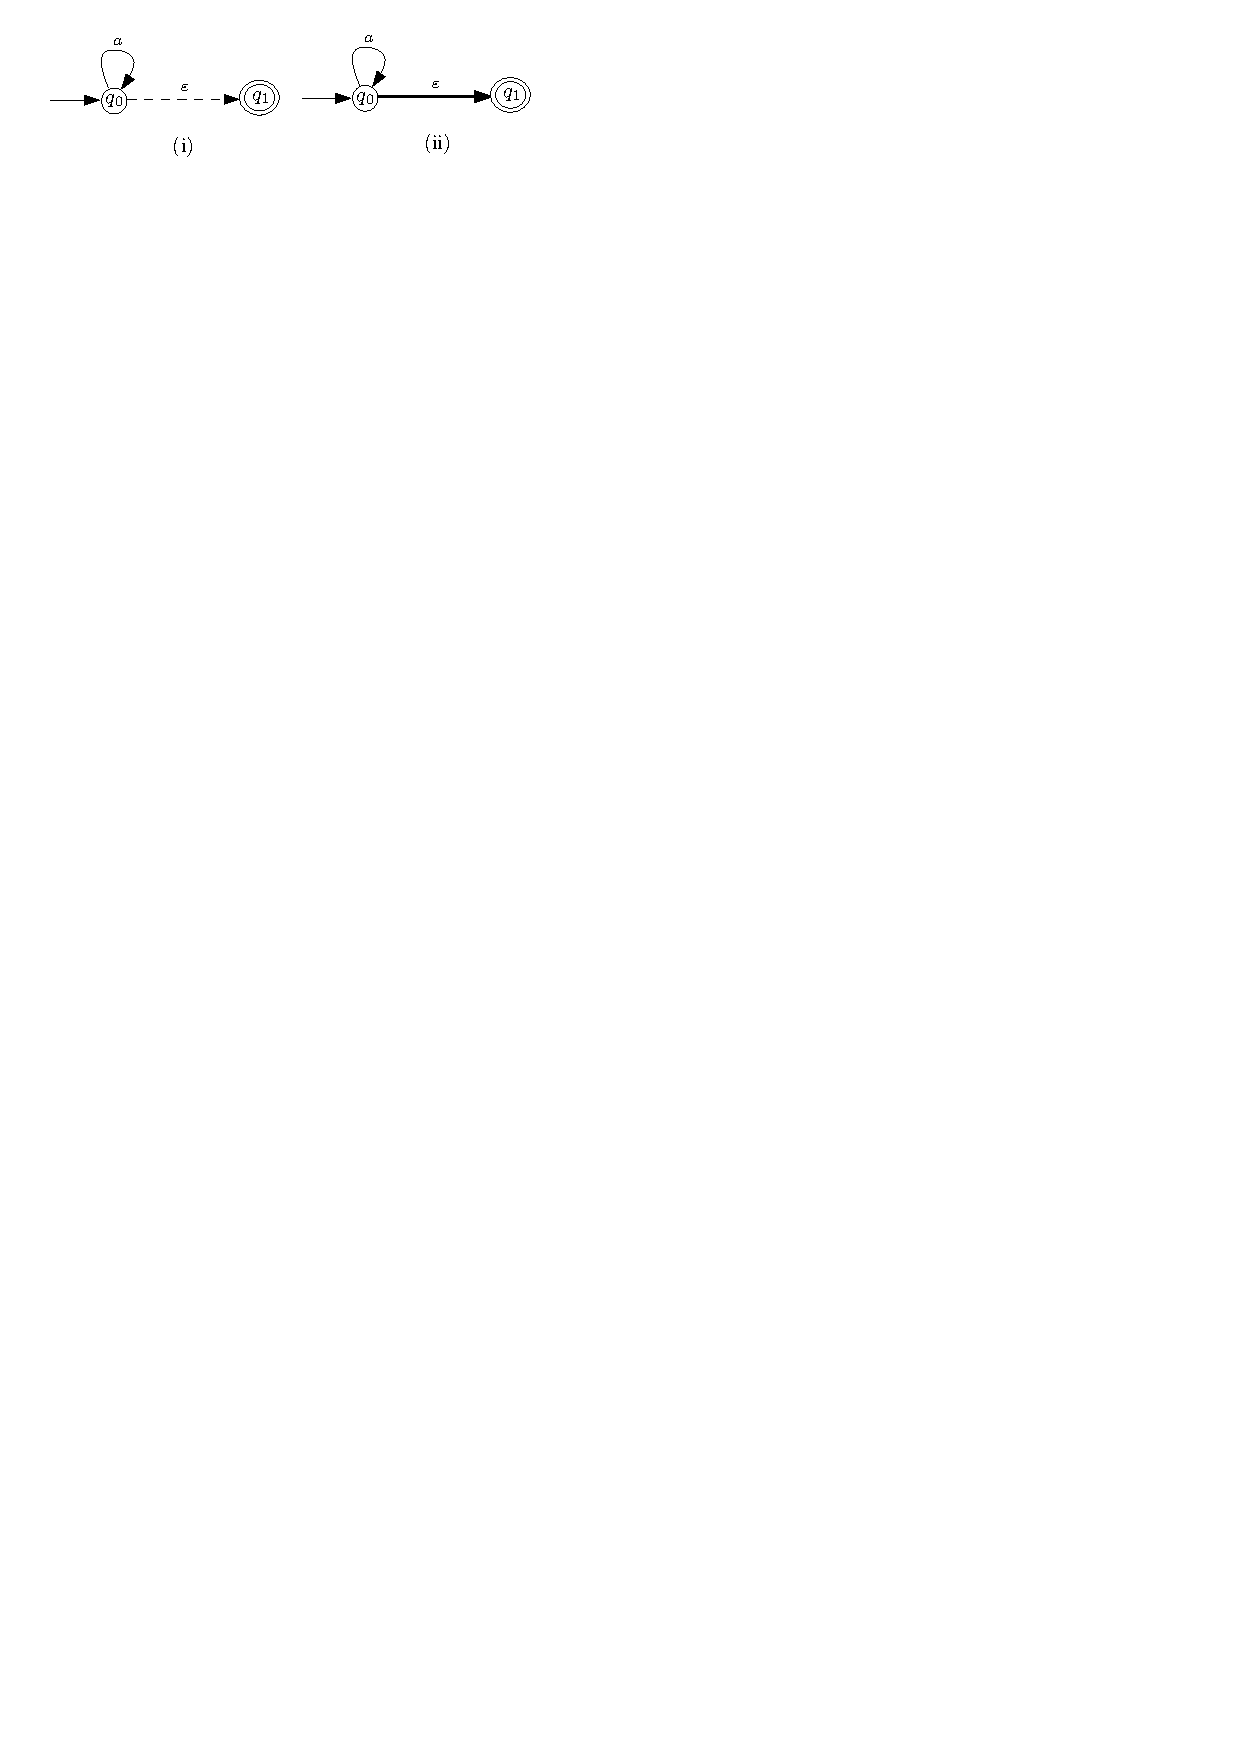
\includegraphics[width=0.6\textwidth]{pfa.pdf}
%\caption{The PFAs for $a^\ast$ and $a^{\ast?}$}
%\label{fig-pfa}
%\end{figure}
%\end{example}
%}
%%%%%%%%% The old example %%%%%%%%%

%\begin{remark}
%Remark that PFAs in Definition~\ref{def-pfa} are different from pNFAs in \cite{BM17} in the sense that the state set in a pNFA is partitioned into two disjoint subsets and the non-$\varepsilon$-transitions are deterministic, while this is not the case in PFAs. Therefore, PFAs are slightly more flexible than pNFAs in \cite{BM17}. We choose this definition of PFAs as a more natural extension of FAs. 
%\end{remark}

%The priorities of PFAs are used to model the greedy and non-greedy semantics of $\regexp$. %, as we shall see in Section~\ref{construction:pnfa}.

%%%%%%%%%%%%%%%%%%%%%%%%%%%%%%%%%%%%%%%%%%%%%%%%%%%%%%%%%%%%%%%%%%%%%%%%%%%%%%%%%%%%%%%%%%%%%%%%%%
%PSST
%%%%%%%%%%%%%%%%%%%%%%%%%%%%%%%%%%%%%%%%%%%%%%%%%%%%%%%%%%%%%%%%%%%%%%%%%%%%%%%%%%%%%%%%%%%%%%%%%%%%%%%


%a new class of transducers that combine prioritized finite-state automata \cite{BM17} %which combines the expressive power of 
%and streaming string transducers \cite{AC10,AD11}.

For a finite set $Q$, let $\overline{Q} = \bigcup_{n\in \Nat}\{ (q_1, \ldots, q_n) \mid \forall i \in [n], q_i \in Q \wedge \forall i,j \in[n], i \neq j \rightarrow q_i \neq q_j \}$. Intuitively, $\overline{Q}$ is the set of sequences of non-repetitive elements from $Q$. In particular, the empty sequence $() \in \overline{Q}$. Note that the length of each sequence from $\overline{Q}$ is bounded by  $| Q |$. For a sequence $P = (q_1, \ldots, q_n) \in \overline{Q}$ and  $q \in Q$, we write $q \in P$ if  $q = q_i$ for some $i \in [n]$. Moreover, for $P_1 = (q_1, \ldots, q_m) \in \overline{Q}$ and $P_2 = (q'_1, \ldots, q'_n) \in \overline{Q}$, we say $P_1 \cap P_2 = \emptyset$ if $\{q_1, \ldots, q_m\} \cap \{q'_1, \ldots, q'_n\} = \emptyset$.
    


%%%%%%%%%%%%%%%%%%%%%%%%%%%%%%%%%%%%%%%%%%%%
%%%%%%%%%%%%%%%%%%%%%%%%%%%%%%%%%%%%%%%%%%%%
%\OMIT{
%\begin{definition}[Prioritized Streaming String Transducers]
%A \emph{prioritized streaming string transducer} (PSST) is a tuple $\psst = (Q, \Sigma, X, \delta, \tau, E, q_0, F)$, where $Q$ is a
%finite set of states, $\Sigma$ is the input and output alphabet such that $\nullchar \not \in \Sigma$, $X$ is a finite set of variables, $\delta \in Q \times \Sigma \rightarrow \overline{Q}$, $\tau \in Q \rightarrow \overline{Q} \times \overline{Q}$, $E$ is a partial function from $Q \times \Sigma^\varepsilon \times
%  Q$ to $X \rightarrow \{\nullchar\} \cup (X \cup \Sigma)^{\ast}$, i.e. the set of assignments,
%   $q_0 \in Q$ is the initial state, and $F$ is a partial function
%  from $Q$ to $(X \cup \Sigma)^{\ast}$.
%\end{definition}
%}
%%%%%%%%%%%%%%%%%%%%%%%%%%%%%%%%%%%%%%%%%%%%
%%%%%%%%%%%%%%%%%%%%%%%%%%%%%%%%%%%%%%%%%%%%


\begin{definition}[Prioritized Streaming String Transducers]
A \emph{prioritized streaming string transducer} (\PSST) is a tuple $\psst = (Q, \Sigma, X, \delta, \tau, E, q_0, F)$, where 
\begin{itemize}
\item $Q$ is a finite set of states, 
\item $\Sigma$ is the input and output alphabet, 
\item $X$ is a finite set of string variables, 
\item $\delta \in Q \times \Sigma \rightarrow \overline{Q}$ defines the non-$\varepsilon$ transitions as well as their priorities (from highest to lowest),
% 
\item $\tau \in Q \rightarrow \overline{Q} \times \overline{Q}$ such that for every $q \in Q$, if $\tau(q) = (P_1; P_2)$, then $P_1 \cap P_2 = \emptyset$, (Intuitively, $\tau(q)=(P_1; P_2)$ specifies the $\varepsilon$-transitions at $q$, with the intuition that the $\varepsilon$-transitions to the states in $P_1$ (resp. $P_2$) have higher (resp. lower) priorities than the non-$\varepsilon$-transitions out of $q$.)
\item $E$ associates with each transition a string-variable assignment function, i.e., $E$ is partial function from $Q \times \Sigma^\varepsilon \times
  Q$ to $X \rightarrow (X \cup \Sigma)^{\ast}$ such that its domain is the set of tuples $(q, a, q')$ satisfying that either $a \in \Sigma$ and $q' \in \delta(q, a)$ or $a = \varepsilon$ and $q' \in \tau(q)$,
\item  $q_0 \in Q$ is the initial state, and
\item  $F$ is the output function, which is a partial function from $Q$ to $(X \cup \Sigma)^{\ast}$.
\end{itemize}
\end{definition}
%
For $\tau(q)=(P_1; P_2)$, we will use $\pi_1(\tau(q))$ and $\pi_2(\tau(q))$ to denote $P_1$ and $P_2$ respectively.  
%With slight abuse of notation, we write $q\in (P_1; P_2)$ for $q\in P_1\cup P_2$. 
%Intuitively, $\tau(q)=(P_1; P_2)$ specifies the $\varepsilon$-transitions at $q$, with the intuition that the $\varepsilon$-transitions to the states in $P_1$ (resp. $P_2$) have higher (resp. lower) priorities than the non-$\varepsilon$-transitions out of $q$.
The size of $\psst$, denoted by $|\psst|$, is defined as $\sum \limits_{(q, a, q') \in \dom(E)} \sum \limits_{x \in X} |E((q, a, q'))(x)|$, where $|E((q, a, q'))(x)|$ is the length of $E(q, a, q')(x)$, i.e., the number of symbols from $X \cup \Sigma$ in it. A PSST $\psst $ is said to be \emph{copyless} if for each transition $(q, a, q')$ in $\psst$ and each $x \in X$, $x$ occurs in $(E(q, a, q')(x'))_{x' \in X}$ at most once. A PSST $\psst$ is said to be \emph{copyful} if it is not copyless. For instance, if $X = \{x_1, x_2\}$ and $E(q, a, q')(x_1) = x_1$ and $E(q, a, q')(x_2) = x_1a$ for some transition $(q, a, q')$, then $\psst$ is copyful. 

A run of $\psst$ on a string $w$ is a sequence $q_0 a_1 s_1 q_1 \ldots a_m s_m q_m$ such that
\begin{itemize}
%\item $q_m \in F$,
%
\item for each $i \in [m]$, 
\begin{itemize}
\item either $a_i \in \Sigma$, $q_i \in \delta (q_{i-1}, a_i)$, and $s_i = E (q_{i - 1}, a_i, q_i)$, 
\item or $a_i = \varepsilon$, $q_i \in \tau(q_{i-1})$ and $s_i = E (q_{i - 1}, \varepsilon, q_i)$,
\end{itemize}

%\item for every subsequence $q_i a_{i+1} s_{i+1} q_{i+1} \ldots a_{j} s_j q_j$ such that  $i < j$ and $a_{i+1} = \cdots = a_j = \varepsilon$, it holds that $q_i, \ldots, q_j$ are mutually distinct. (Intuitively, loops of $\varepsilon$-transitions are forbidden.) 
\item for every subsequence $q_i a_{i+1} s_{i+1} q_{i+1} \ldots a_{j} s_j q_j$ such that  $i < j$ and $a_{i+1} = \cdots = a_j = \varepsilon$,  it holds that each $\varepsilon$-transition occurs at most once in it, namely, for every $k, l: i \le k < l < j$, $(q_k, q_{k+1}) \neq (q_l, q_{l+1})$.
\end{itemize}
Note that it is possible that $\delta(q, a) = ()$, that is, there is no $a$-transition out of $q$. 
From the assumption that each $\varepsilon$-transition occurs at most once in a sequence of $\varepsilon$-transitions, we deduce that given a string $w$, the length of a run of $\psst$ on $w$, i.e. the number of transitions in it, is $O(|w||\psst|)$. 

%A run of $\psst$ is the sequence $q_0 a_1 s_1 q_1 \ldots a_m s_m q_m$, where $F (q_m)$ is defined and for each $i \in [m], q_i \in \delta (q_{i-1}, a_i)$ and $s_i = E (q_{i - 1}, a_i, q_i)$. 
For any pair of runs $R = q_0 a_1 s_1 \ldots a_m s_m q_m$ and $R' = q_0 a'_1
  s_1' \ldots a'_n s_n' q_n'$ such that $a_1 \ldots a_m = a'_1 \ldots a'_n$, we say that $R$ is of a higher priority over $R'$ if 
\begin{itemize}
	\item either $R'$ is a prefix of $R$ (in this case, the transitions of $R$ after $R'$ are all $\varepsilon$-transitions), 
	%
	\item or there is an index $j$ satisfying one of the following constraints:
	\begin{itemize}
		\item $q_0 a_1 q_1 \ldots q_{j-1} a_j = q_0 a'_1 q'_1 \ldots q'_{j-1} a'_j$, $q_j \neq q'_j$, $a_j \in \Sigma$, and $\delta (q_{j - 1}, a_j) =(\ldots, q_j, \ldots, q_j', \ldots)$,
		%
		\item $q_0 a_1 q_1 \ldots q_{j-1} a_j = q_0 a'_1 q'_1 \ldots q'_{j-1} a'_j$, $q_j \neq q'_j$, $a_j  = \varepsilon$,  and one of the following conditions holds: (i) $\pi_1(\tau(q_{j - 1})) = (\ldots, q_j, \ldots, q_j', \ldots)$, (ii) $\pi_2(\tau(q_{j - 1})) = (\ldots, q_j, \ldots, q_j', \ldots)$, or (iii) $q_j \in \pi_1(\tau(q_{j - 1}))$ and $q'_j \in \pi_2(\tau(q_{j-1}))$, 
		%
		\item $q_0 a_1 q_1 \ldots q_{j-1}  = q_0 a'_1 q'_1 \ldots q'_{j-1} $, $a_j  = \varepsilon$, $a'_j  \in \Sigma$, $q_j \in \pi_1(\tau(q_{j - 1}))$, and $q'_j \in \delta(q_{j-1}, a'_j)$, 
		%
		\item $q_0 a_1 q_1 \ldots q_{j-1}  = q_0 a'_1 q'_1 \ldots q'_{j-1} $, $a_j  \in \Sigma$, $a'_j  = \varepsilon$, $q_j \in \delta(q_{j - 1}, a_j)$, and $q'_j \in \pi_2(\tau(q_{j-1}))$.
	\end{itemize}
\end{itemize}
  
  
  % $p \neq p'$ and, for the smallest index $j$ with $q_j \neq q_j'$,
 % $\delta (q_{j - 1}, a_j) = \ldots q_j \ldots q_j' \ldots$
  
An \emph{accepting} run of $\psst$ on $w$ is a run of $\psst$ on $w$, say $R = q_0 a_1 s_1 \ldots a_m s_m q_m$, such that 1) $F(q_m)$ is defined, 2)  $R$ is of the highest priority among those runs satisfying 1). The output of $\psst$ on $w$, denoted by $\psst(w)$, is defined as $\eta_m(F(q_m))$, where $\eta_0(x) = \varepsilon$ for each $x \in X$, and $\eta_{i}(x) = \eta_{i-1}(s_{i}(x))$ for every $1 \le i \le m$ and $x \in X$. Note that here we abuse the notation $\eta_m(F(q_m))$ and $\eta_{i-1}(s_{i}(x))$ by taking a function $\eta$ from $X$ to $\Sigma^*$ as a function from $(X \cup \Sigma)^*$ to $\Sigma^*$, which maps each $x \in X$ to $\eta(x)$ and each $a \in \Sigma$ to $a$. If there is no accepting run of $\psst$ on $w$, then $\psst(w) = \bot$, that is, the output of $\psst$ on $w$ is undefined. The string relation defined by $\psst$, denoted by $\cR_\psst$,  is 
$\{(w, \psst(w)) \mid w \in \Sigma^\ast, \psst(w)  \neq \bot\}$.
%Note that in the definition of $\cR_\psst$ above, the inputs of $\psst$ whose outputs are in $(\Sigma \cup \{\nullchar\})^* \setminus (\Sigma^* \cup \{\nullchar\})$ are ignored.


\begin{example}
The {\PSST} $\cT=(Q, \Sigma, X, \delta, \tau, E,  q_{0}, F)$ to extract the match of the first capturing group for the regular expression \mintinline{javascript}{(\d+)(\d*)} 
%in Example~\ref{exm-plre} 
%
is illustrated in Fig.~\ref{fig-psst-exmp}, where $x_1$ and $x_2$ store the matches of the two capturing groups. More specifically, in $\cT$ we have $\Sigma = \{0,\cdots,9\}$, $X= \{x_1,x_2\}$, $F(q_{4}) = x_1$ denotes the final output, and $\delta, \tau, E$ are illustrated %by the edges 
in Fig.~\ref{fig-psst-exmp}, where the dashed edges denote the $\varepsilon$-transitions of lower priorities than the non-$\varepsilon$-transitions and the symbol $\ell$ denotes the currently scanned input letter. For instance, for the state $q_2$, $\delta(q_2, \ell) = (q_2)$ for $\ell \in \{0,\ldots, 9\}$, $\tau(q_2) = (();(q_3))$, $E(q_2, \ell, q_2)(x_1) = x_1 \ell$, $E(q_2, \ell, q_2)(x_2) = x_2$,  $E(q_2, \varepsilon, q_3)(x_1) = x_1$, and $E(q_2, \varepsilon, q_3)(x_2) = \varepsilon$. Note that the identity assignments, e.g. $E(q_2, \varepsilon, q_3)(x_1) = x_1$, are omitted in Fig.~\ref{fig-psst-exmp} for readability.  For the input string $w$=``2050'', the accepting run of $\cT$ on $w$ %, namely, a run of $\cT$ on $w$ ending at $q_4$ and of the highest priority, 
is 
\[
q_0 \xrightarrow[x_1:=\varepsilon]{\varepsilon} q_1 \xrightarrow[x_1:=x_12]{2} q_2  \xrightarrow[x_1:=x_10]{0} q_2  \xrightarrow[x_1:=x_15]{5} q_2  \xrightarrow[x_1:=x_10]{0} q_2  \xrightarrow[x_2:=\varepsilon]{\varepsilon} q_3  \xrightarrow{\varepsilon} q_4,
\]
where the value of $x_1$ and $x_2$ when reaching the state $q_4$ are ``2050'' and $\varepsilon$ respectively. 
%From $\delta(q_4, \backslash s) = q_5q_{6}$, we know that $q_5$ is prior to $q_6$. 
%Therefore, whenever $\cT_{\sf nameReg}$ reads $\backslash$s at the state $q_3$,  it will choose to go the state $q_5$ greedily, unless this choice would lead to the nonacceptance (in this case, $q_6$ will be chosen). 

\begin{figure*}[ht]
\centering
%\rule{\linewidth}{0cm}
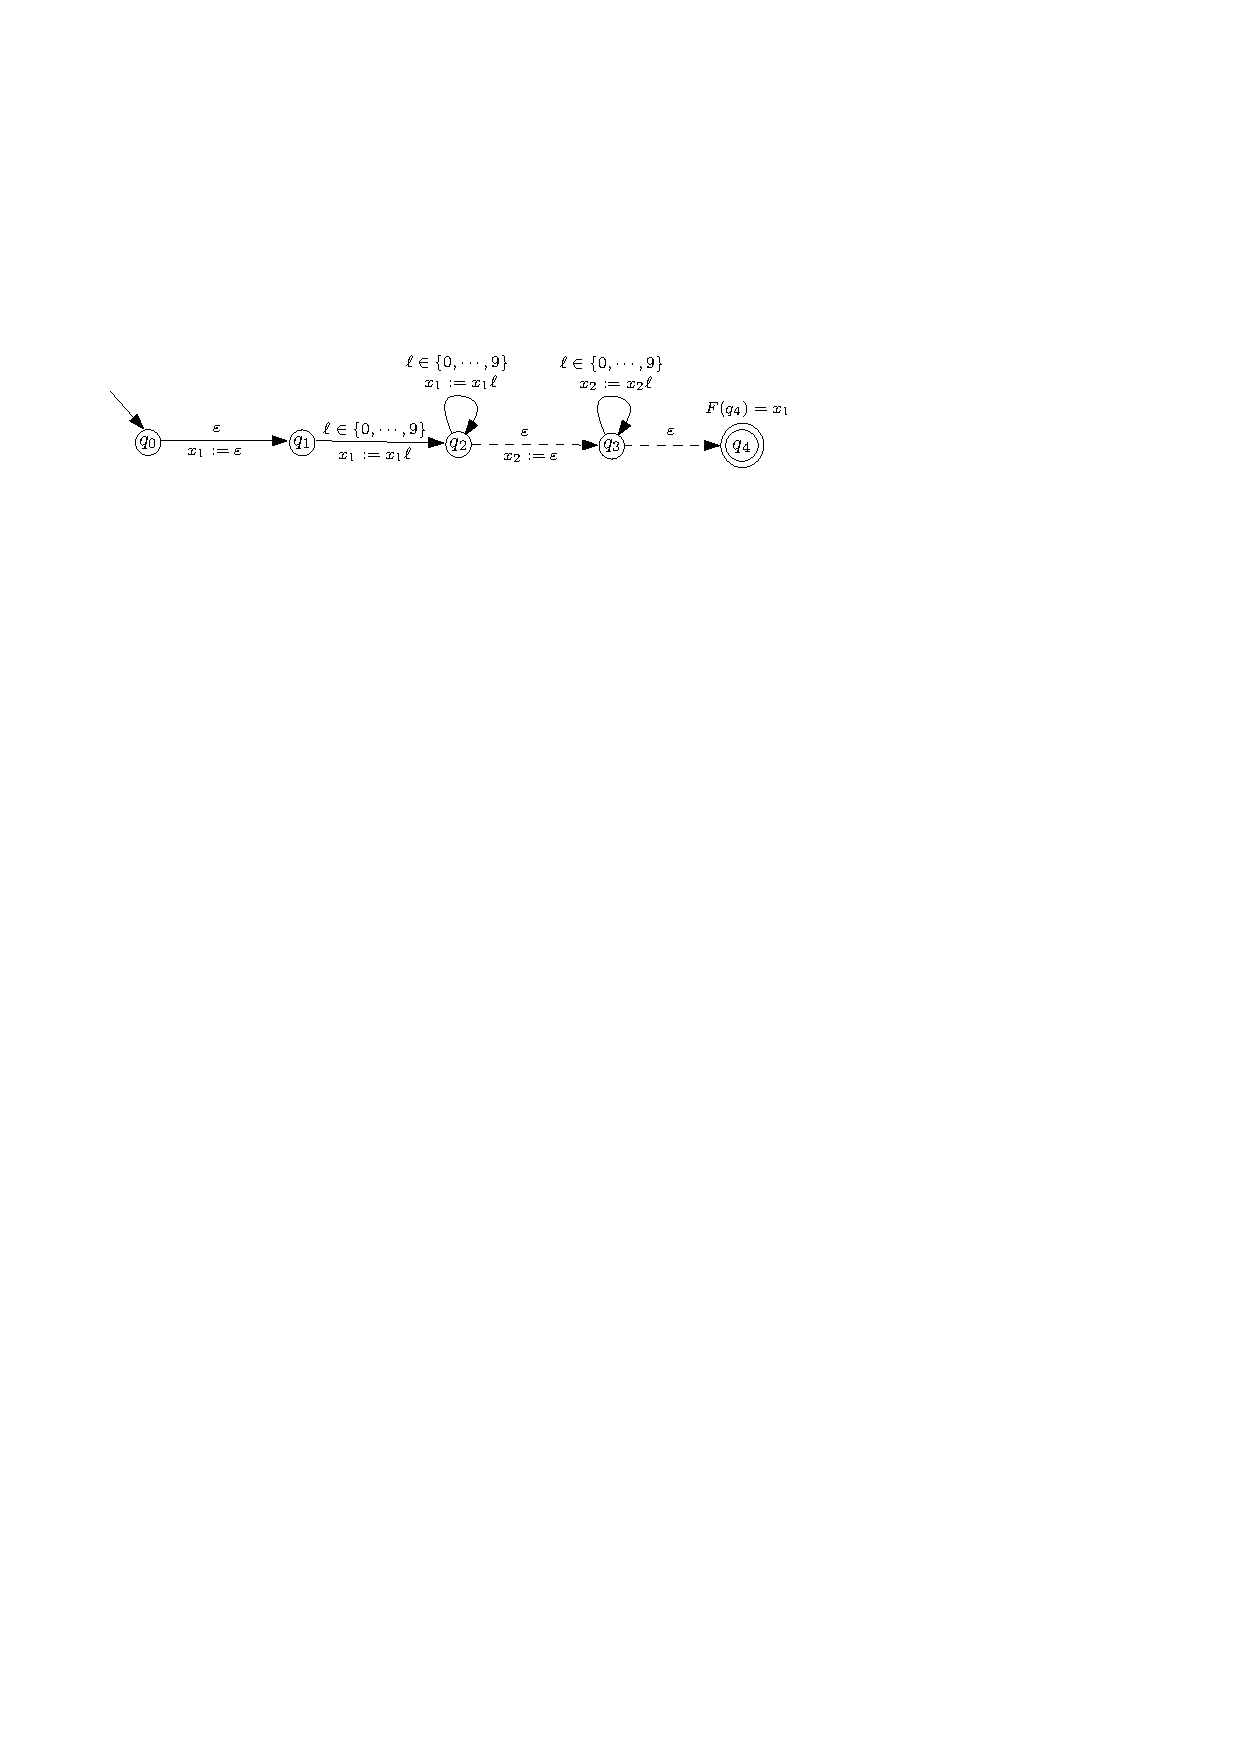
\includegraphics[width=0.8\textwidth]{psst-exmp-decimal.pdf}
\caption{The PSST $\cT$: Extract the matching of the first capturing group in ($\backslash$d+)($\backslash$d*)}
\label{fig-psst-exmp}
%\vspace{-4mm}
\end{figure*}
\end{example}


  
%  $\tmop{Out} (r) =
%  s_{\varepsilon} \circ s_1 \circ s_2 \ldots s_n \circ F (q_n)$ where
%  $s_{\varepsilon}$ is the empty substitution which maps all variables to
%  $\varepsilon$.
  

% Note that in the definition of \NSST, there is no \emph{copyless} restriction.






%%%%%%%%%%%%%%%%%%%%%%%%%%%%%%%%%%%%%%%%%%

\subsection{Defining the Semantics of \regexp-String Matching by PSSTs} \label{sect:regextopsst}


%!TEX root = main.tex



%We are ready to define prioritized streaming string transducers. 
%In the definition, 
%
%The special symbol $\nullchar$ is introduced to capture the situation that $\extract_{i,e}(x)$ returns $\nullchar$, i.e. $x \in \Lang(e)$ but the $i$-th capturing group of $e$ is not matched.
%

%\paragraph{Semantics}
 
%We now define the formal semantics of $\regexp$. Traditionally, regular expressions are interpreted as a regular language, i.e., a set of strings, which can be defined inductively in a rather straightforward way. In our case when the regular expression is used in string constraints arisen from analysis of programming language such as JavaScript, %owing to the introduction of greedy/lazy semantics,  
%what we need is not only the language denoted by the regular expression, but also the intermediate result when parsing a string against the given regular expression. This is especially the case when the capturing group is involved. As a result, we need a more operational (as opposed traditional denotational) account of the semantics for regular expression. To this end, we harness an extension of finite-state automata with priorities, which \emph{defines} how a string is accepted by the given regular expression. We start with the standard finite-state automaton.  
 
We now define the formal semantics of the regex-string matching for $\pcre$. 
The semantics is defined by recursively constructing PSSTs out of {\pcre}s.
 

In \cite{BDM14,BM17}, a construction from regular expressions to prioritized finite transducers (abbreviated as PFT) was given. The construction therein is a variant of the classical Thompson construction from regular expressions to nondeterministic finite automata \cite{Thompson68}. In particular, the size of the constructed PFT is linear in the size of the given regular expression. 
%

One may tempt to believe that the construction in \cite{BDM14,BM17} can be easily adapted to construct PSSTs out of {\pcre}s. 
%
Nevertheless, the construction in \cite{BDM14,BM17} works only for regular expressions where all the subexpressions $e^*$ or $e^{*?}$ satisfy that the language defined by $e$ does \emph{not} contain the empty string, moreover, the construction was not validated against the actual semantics of regex-string matching in programming languages. 
%
In comparison, our goal here is to have a construction that \emph{works for arbitrary {\pcre}s and is consistent with the actual semantics of  regex-string matching in Javascript}. It turns out that our construction of PSSTs out of {\pcre}s in the sequel requires some new ideas and is considerably different from that in  \cite{BDM14,BM17}. In particular, the size of the constructed PSST can be \emph{exponential} in the size of the given regular expression in the worst case.

%\subsection{Semantics of \regexp[\sf CG]}
%In this section, we give one of the many semantics of \regexp[\sf CG], which we will utilize for $\replaceall$.
%For two indexed $\regexp$s $e$ and $e'$, we say $e'$ is a \emph{subexpression} of $e$,
%if one of the following conditions holds: 1) $e'=e$, 2) $e = [e_1 \cdot e_2]$ or $[e_1 + e_2]$, and $e'$ is a subexpression of $e_1$ or $e_2$, 3) $e = [e^?], [e^{??}], [e_1^{\ast}]$, $[e_1^{+}]$, $[e_1^{\ast?}]$, $[e_1^{+?}]$, $e_1^{\{m_1, m_2\}}$, $e_1^{\{m_1, m_2\}?}$ or $(_n e_1)_n$, and $e'$ is a subexpression of $e_1$. We use $S(e)$ to denote the set of all subexpressions of $e$. %\tl{is there a difference between $[e_1\cdot e_2]$ and $e_1 e_2$?}
%
% 
%By a mutual induction on $|w|$ and $|e|$, we can show that $|\cM_{w}(e)|$, the size of $\cM_{w}(e)$, is at most $|w||e|$.  

%\begin{example}\label{exmp-regex-match-tree}
%	Let $w= 0250$ and $e = [[([\Gamma^+])\concat .?] \concat ([\Gamma^*])]$ where $\Gamma = \{0,1,\cdots,9\}$. Note that $e$ is essentially {\tt decimalReg} in the motivating example. Then $\cM_{w}(e) = \{T_1,T_2,T_3, T_4\}$ as illustrated in Figure~\ref{fig-regex-semantics-decimal}(i), (ii), (iii), and (iv), where the match trees rooted at $(0, \Gamma)$, $(2, \Gamma)$, and $(5, \Gamma)$ are omitted. % to avoid tediousness.
%	\begin{figure}[htb]
%		\centering
%		%\rule{\linewidth}{0cm}
%		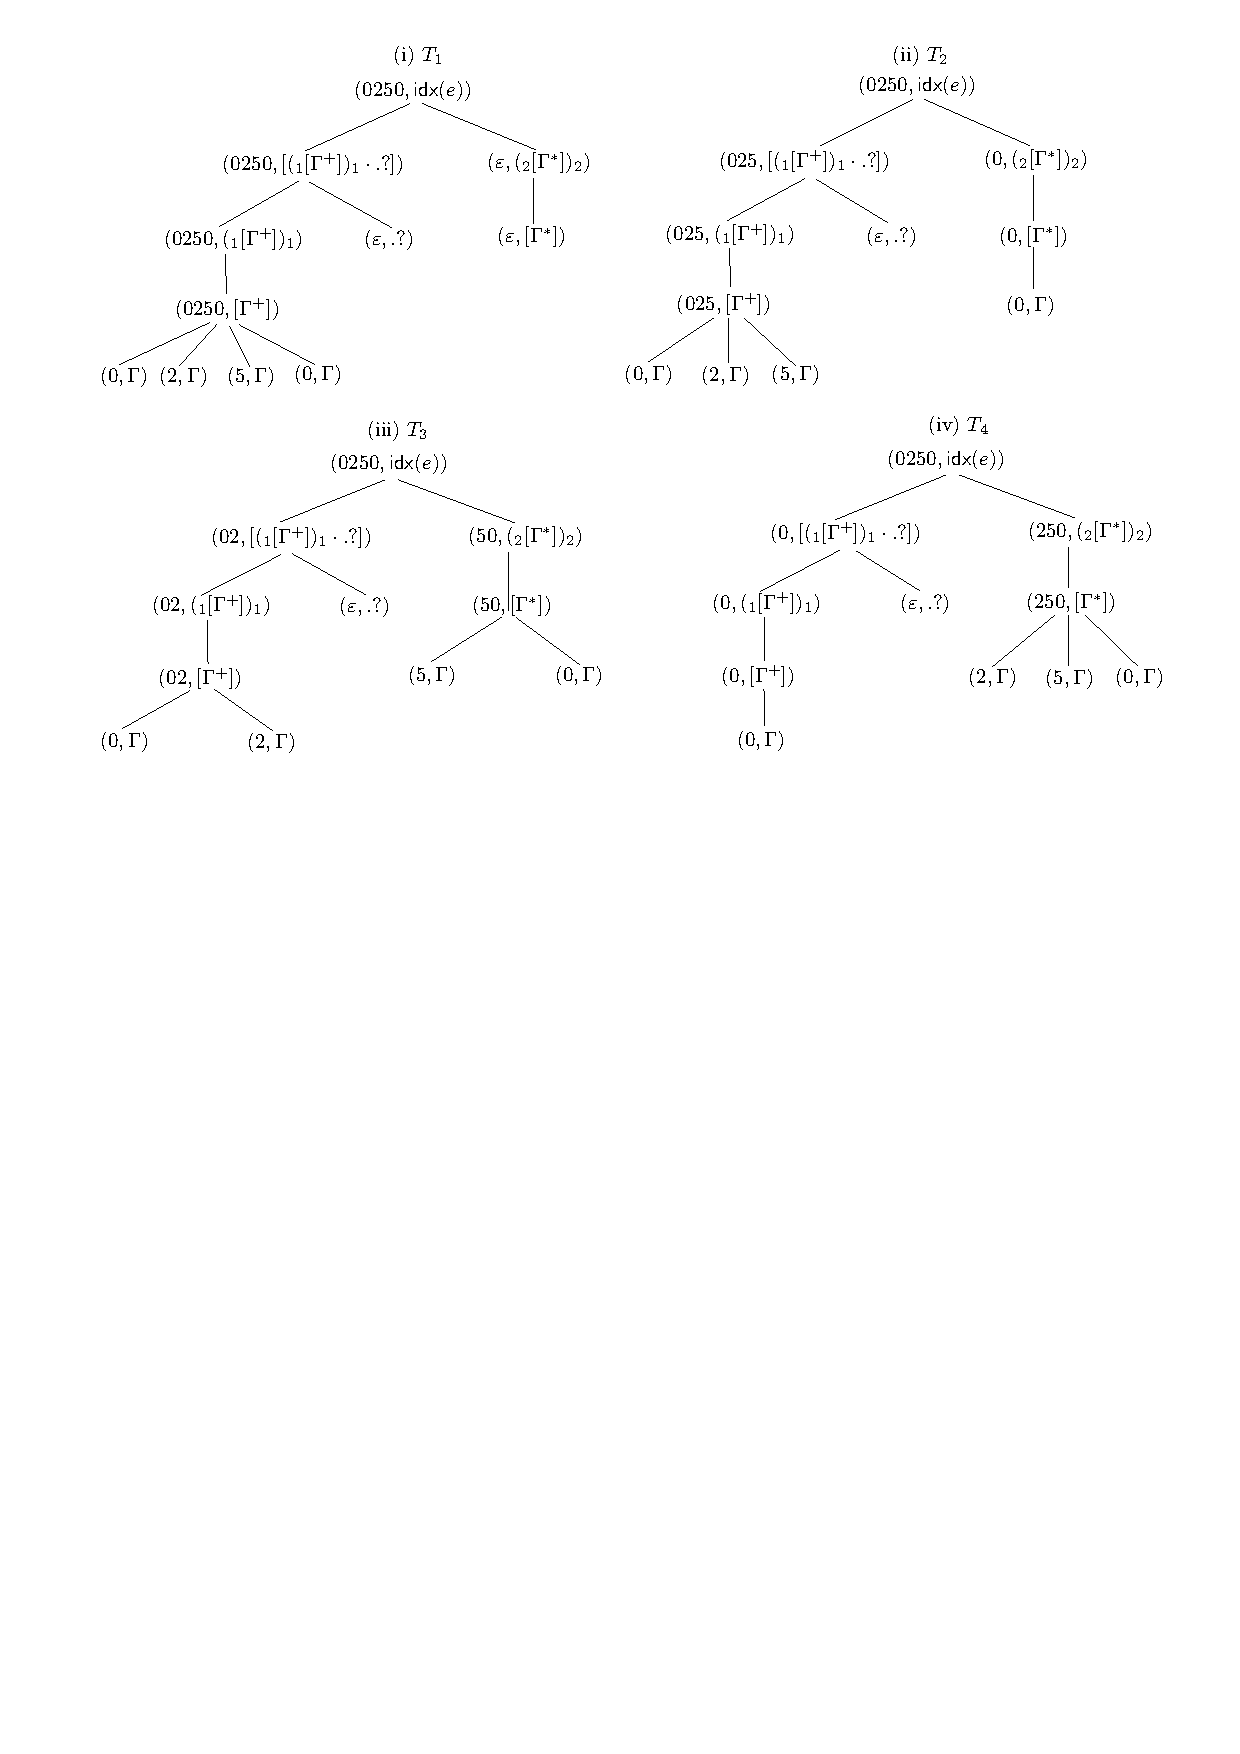
\includegraphics[width=1\textwidth]{regex-semantics-decimal.pdf}
%		\caption{Match trees of $e=[[([\Gamma^+])\concat .?] \concat ([\Gamma^*])]$ to $w= 0250$}
%		\label{fig-regex-semantics-decimal}
%		
%	\end{figure}
%	%\Blindtext
%\end{example}

 
 
%
%\begin{example}\label{exmp-regex-semantics}
%	Let us continue Example~\ref{exmp-regex-match-tree}.  In Fig.~\ref{fig-regex-semantics-decimal}, we have $(T_1)_{(0250, [\Gamma^+])} >_{(w, \idxexp(e))} (T_2)_{(025, [\Gamma^+])}$, since $(0, \Gamma)(2, \Gamma)(5,\Gamma)$ is a proper prefix of $(0, \Gamma)(2, \Gamma)(5,\Gamma)(0, \Gamma)$. Then we deduce that $(T_1)_{(0250, (_1[\Gamma^+])_1)} >_{(w, \idxexp(e))} (T_2)_{(025, (_1[\Gamma^+])_1)}$. Consequently, $(T_1)_{(0250, [(_1[\Gamma^+])_1 \concat .?])} >_{(w, \idxexp(e))} (T_2)_{(025,  [(_1[\Gamma^+])_1 \concat .?])}$ and $T_1 >_{(w, \idxexp(e))} T_2$. Similarly, we have $T_2 >_{(w, \idxexp(e))} T_3$ and $T_3 >_{(w, \idxexp(e))} T_4$. Therefore, $T_1$ is the accepting match of $e$ to $w$, where the first and second capturing group of $e$ are matched to $0250$  and $\varepsilon$ respectively. 
%	%\Blindtext
%\end{example}

%\begin{remark}
%	Our semantics of $\regexp$ follows the 11th Edition of the ECMAScript specification (ES11 for short) \cite{ECMAScript11}, with a focus on the non-commutative union, the greedy/lazy semantics of Kleene star/plus, as well as capturing groups and backreferences.
%	In comparison, POSIX regular expressions require the leftmost and longest match of regular expressions, which we leave as future work.
%\end{remark}


% some examples

%  e = b(a*)a*
%  
%  e' = b(a*?)a*

%\begin{figure}[ht]
%\centering
%\rule{\linewidth}{0cm}
%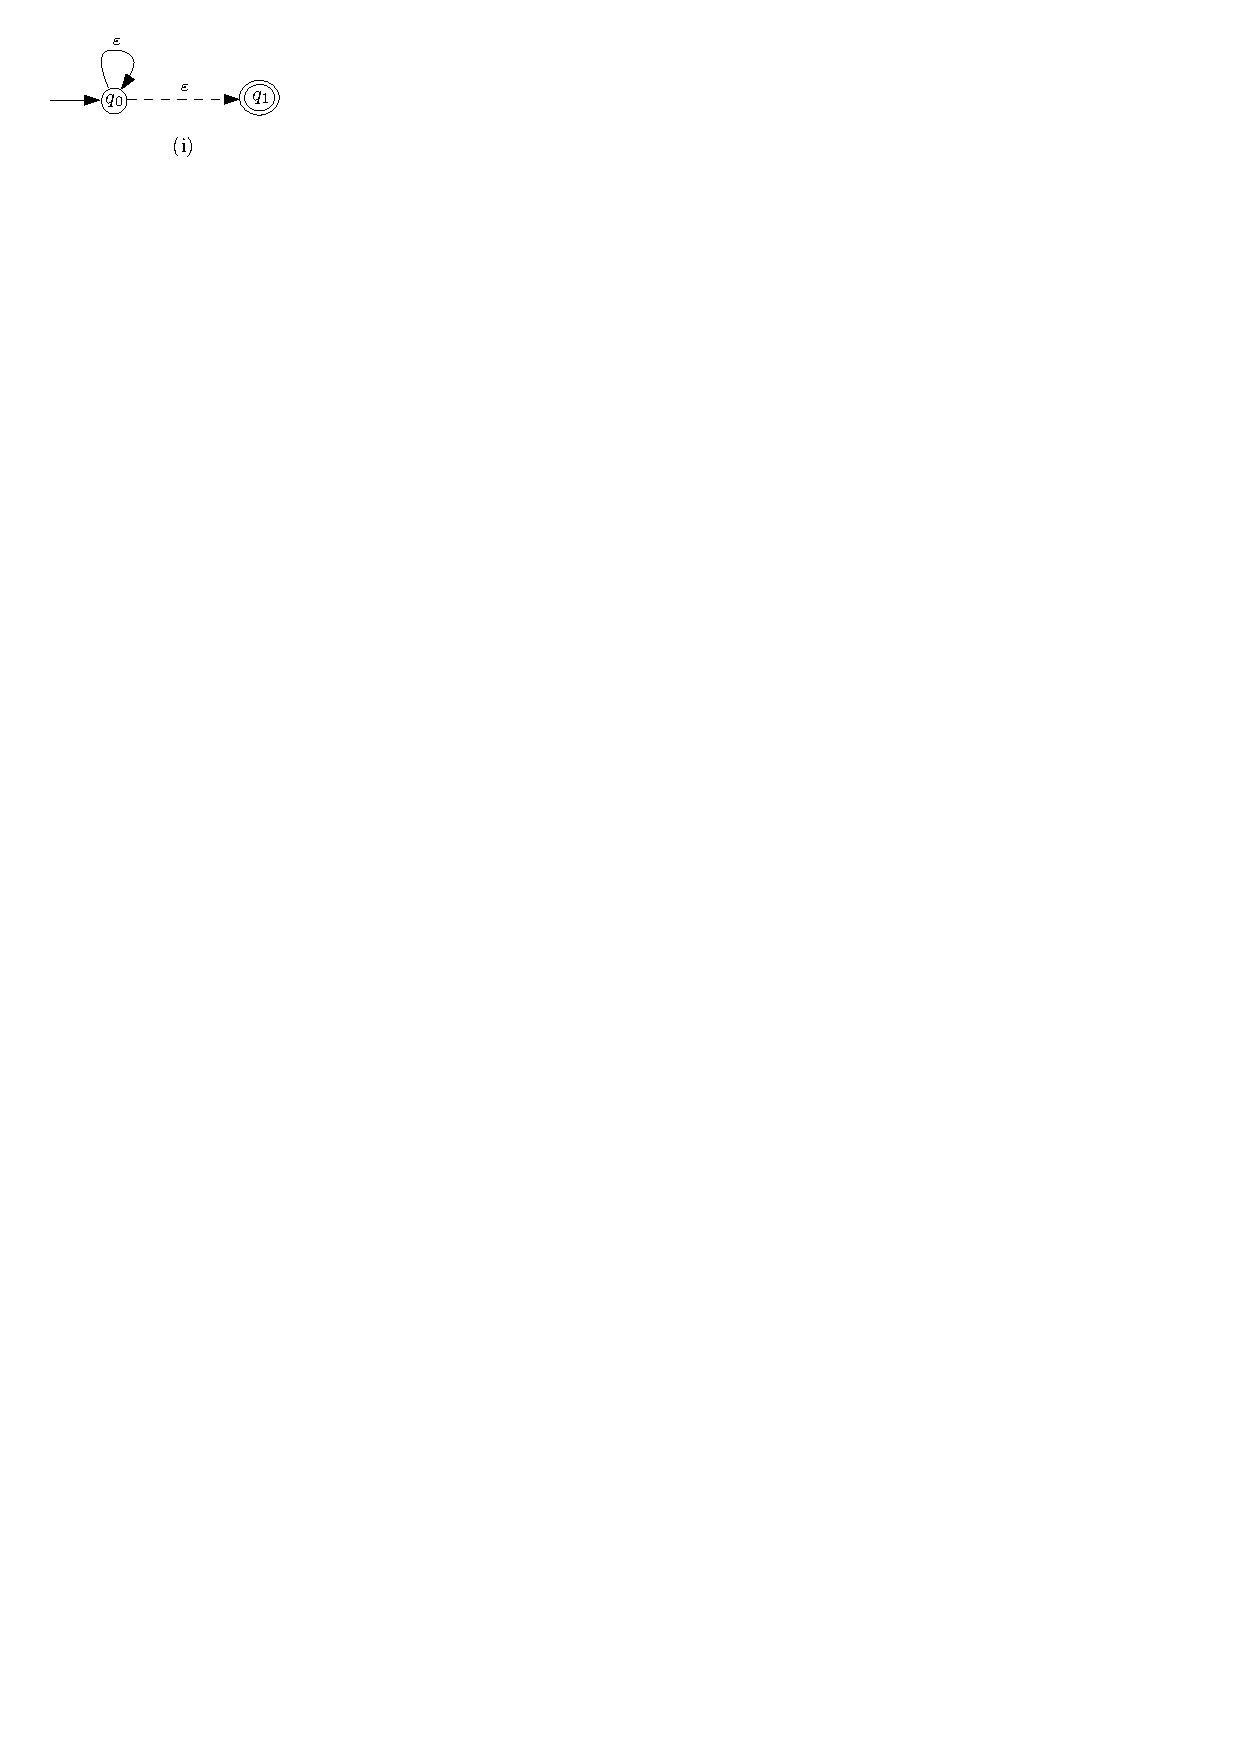
\includegraphics[scale=0.8]{pfa-epsilon-star.pdf}
%\caption{The PFA for $\varepsilon^\ast$}
%\label{fig-pfa-epsilon-star}
%\end{figure}



%%%%%%%%%%%%%%%%%%%%%%%%%%%%%%%%%%%%%%%%%%%%%%%%%%%%%%%%%%%%%%%%%%%%%%%%%%%%%%%%%%%%%%%%%%%%

%We can adapt the PFA construction in \cite{BDM14}, which in turn is a variant of the standard Thompson construction \cite{Thompson68}, and show the following result. 

%\begin{proposition}\label{prop-rwre-to-pfa}

%We associate with each regular expression $e$ a PFA $\cA_e$ and define the semantics of $e$ as the language accepted by $\cA_e$. As expected, the PFA $\cA_e$ is constructed inductively. 

\zhilin{stopped here}

\paragraph{Case $e =\emptyset$} $\cA_e = (\{q_{\emptyset, 0}\}, \Sigma, \emptyset, \delta, \tau, E, q_{\emptyset, 0}, (\emptyset, \emptyset))$, where $\delta(q_{\emptyset, 0}, a) = ()$ for every $a \in \Sigma$; $\tau(q_{\emptyset, 0}) = ((); ())$; $E$ is indeed vacuous.
		

\paragraph{Case $e = \varepsilon$} $\cA_e = (\{q_{\varepsilon, 0}, f_{\varepsilon,0}\}, \Sigma, \{x \}, \delta, \tau, E, q_{\varepsilon,0}, (\{f_{\varepsilon,0}\}, \emptyset))$, 
%
where $\delta(q_{\varepsilon,0}, a) = \delta(f_{\varepsilon,0}, a) = ()$ for every $a \in \Sigma$; $\tau(q_{\varepsilon,0}) = ((f_{\varepsilon,0}); ())$;  $\tau(f_{\varepsilon,0}) = ((); ())$; %for each transition $(q, a, q')$, 
$E(q_{\varepsilon,0}, \varepsilon, f_{\varepsilon,0})(x) = \varepsilon$.
		
\paragraph{Case $e = a$} $\cA_e = (\{q_{a,0}, q_{a,1}, f_{a,0}\}, \Sigma, \{x\}, \delta, \tau, E, q_{a,0}, (\emptyset, \{f_{a,0}\}))$, where 
$\delta(q_{a,0}, b) = ()$ for every $b \in \Sigma$, $\delta(q_{a,1}, a) = (f_{a,0})$, $\delta(q_{a,1}, b) = ()$ for every $b \in \Sigma \setminus \{a\}$; 
%
$\tau(q_{a,0}) = ((q_{a,1}); ())$, $\tau(q_{a,1}) = ((); ())$, and $\tau(f_{a,0}) = ((); ())$; 
%
for each transition $(q, a, q')$, $E(q,a,q')(x) =xa$.
%		
\begin{figure}[ht]
			\centering
			%\rule{\linewidth}{0cm}
			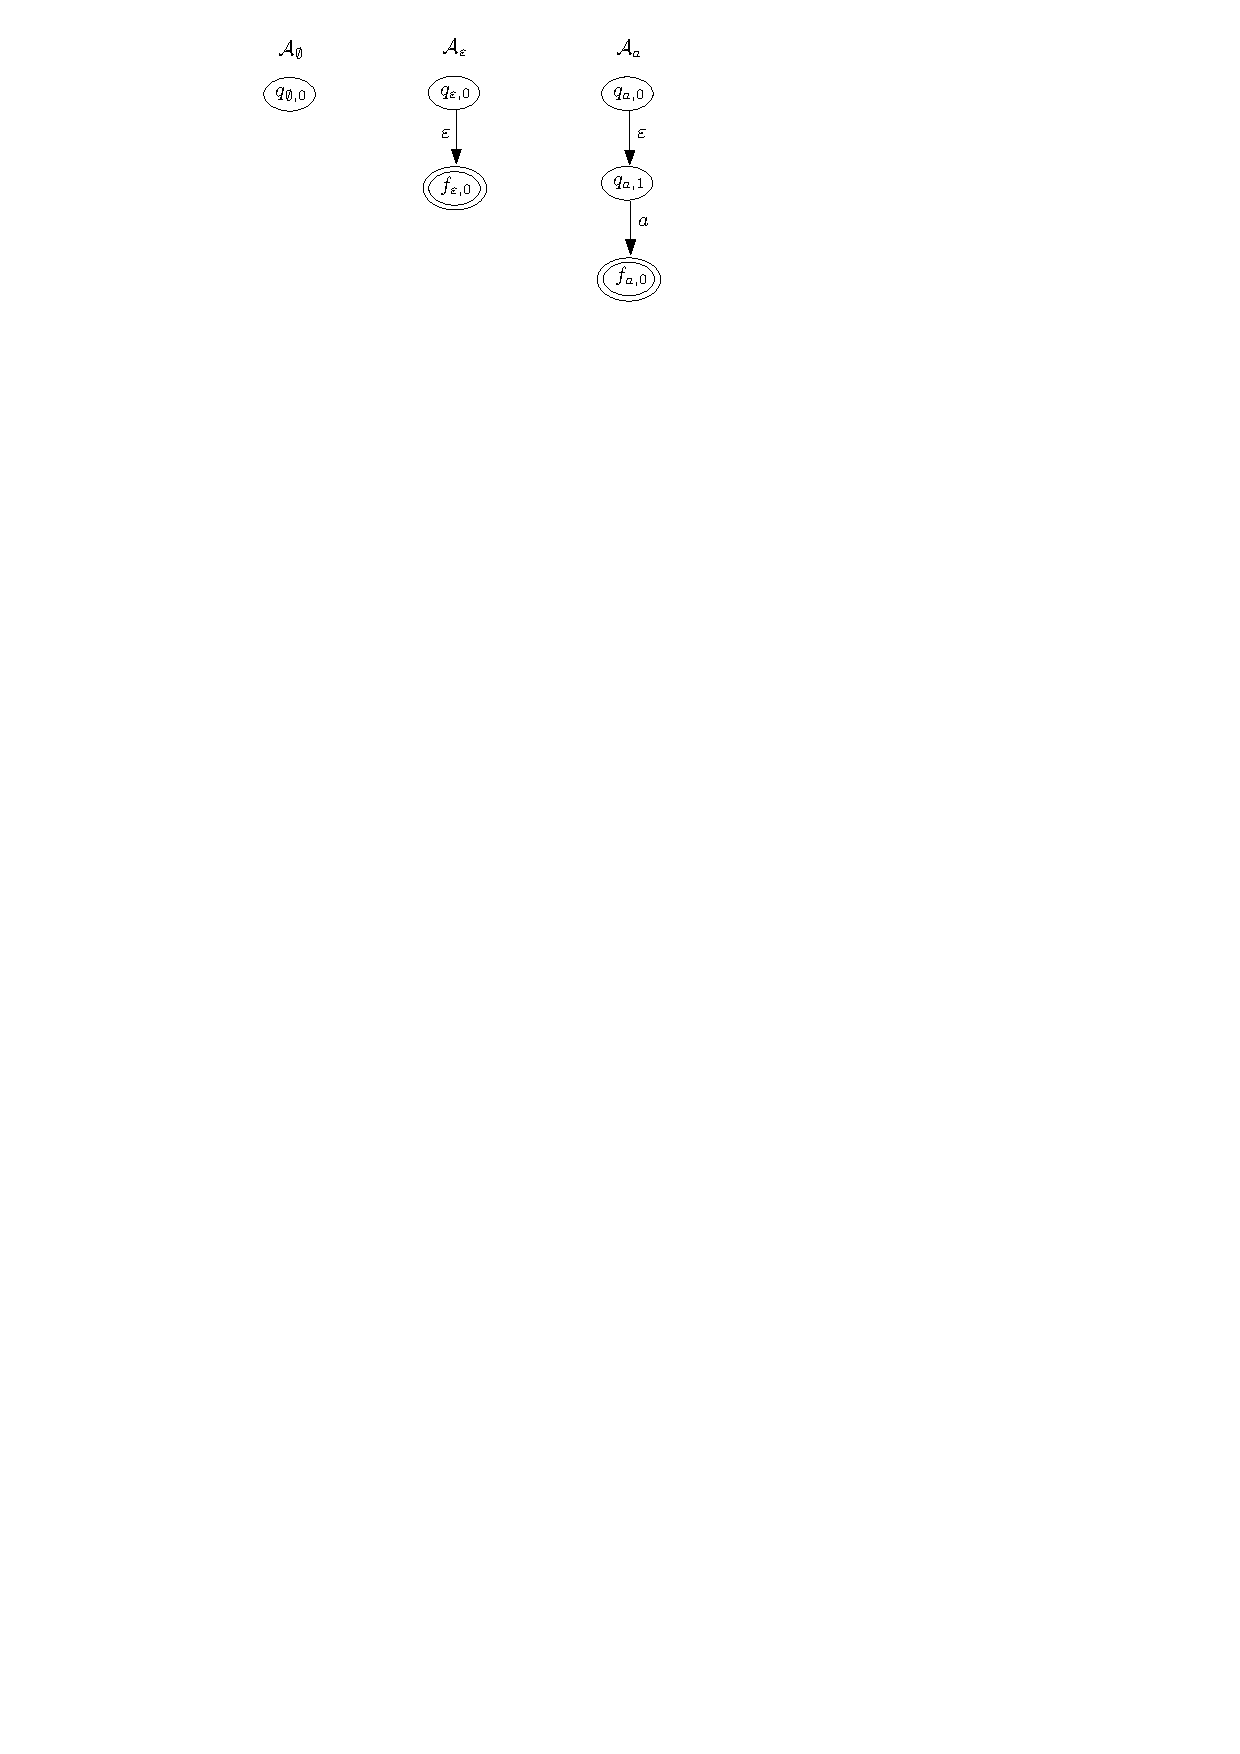
\includegraphics[width = 0.4\textwidth]{reg2pfa-0.pdf}
			\caption{The PFA $\cA_{\emptyset}$, $\cA_{\varepsilon}$, and $\cA_{a}$ }
			\label{fig-reg2pfa-0}
\end{figure}  
%%%%%%%%%%%%%%%%%%%%%%%%%%%%%%%%%%%%%%%%%%%%%%%%%%%%%%%%%%%%%%%%%%%%%%%%%%%%%%%%%%%%%%%%%%%%%%%%%%%%

		
\paragraph{Case $e = (e_1)$} $\cA_e = \cA_{e_1}$.
		

\paragraph{Case $e = [e_1 + e_2]$} Let 
\[\cA_{e_1} = (Q_{e_1}, \Sigma, X_1, \delta_{e_1}, \tau_{e_1}, E_1,  q_{e_1,0}, (F_{e_1,1}, F_{e_1,2}))\] and 
\[\cA_{e_2} = (Q_{e_2}, \Sigma, X_2, \delta_{e_2}, \tau_{e_2}, E_2, q_{e_2,0}, (F_{e_2, 1}, F_{e_2,2}))\] 
 
Then 
\[\cA_e = (Q_{e_1} \cup Q_{e_2} \cup \{q_{e,0}\}, \Sigma, X_1\cup X_2, 
		\delta_e, \tau_e, E, q_{e,0}, (F_{e_1,1} \cup F_{e_2,1}, F_{e_1,2} \cup F_{e_2,2}))\] where  
		\begin{itemize}
			\item $q_{e,0}  \not \in Q_{e_1} \cup Q_{e_2}$, 
			\item $\delta_e(q, a) = \delta_{e_i}(q, a)$ for every $i \in \{1,2\}$, $q \in Q_{e_i}$ and $a \in \Sigma$, 
			$\delta_e(q_{e,0}, a)  = ()$ for every $a \in \Sigma$, 
			%
			\item $\tau_e(q) = \tau_{e_i}(q)$ for every $q \in Q_{e_i}$ ($i =1,2$), $\tau_e(q_{e,0}) = ((q_{e_1,0},q_{e_2,0}); ())$.
			\item for each transition $(q, a, q')$ from $\delta_i$ for $i\in\{1,2\}$, $E(q,a,q')(x) =xa$ and $E(q_{e,0},a,q')(x) =\varepsilon$
		\end{itemize}
Fig.~\ref{fig-reg2pfa-1} depicts the construction.  	
		\begin{figure}[ht]
			\centering
			%\rule{\linewidth}{0cm}
			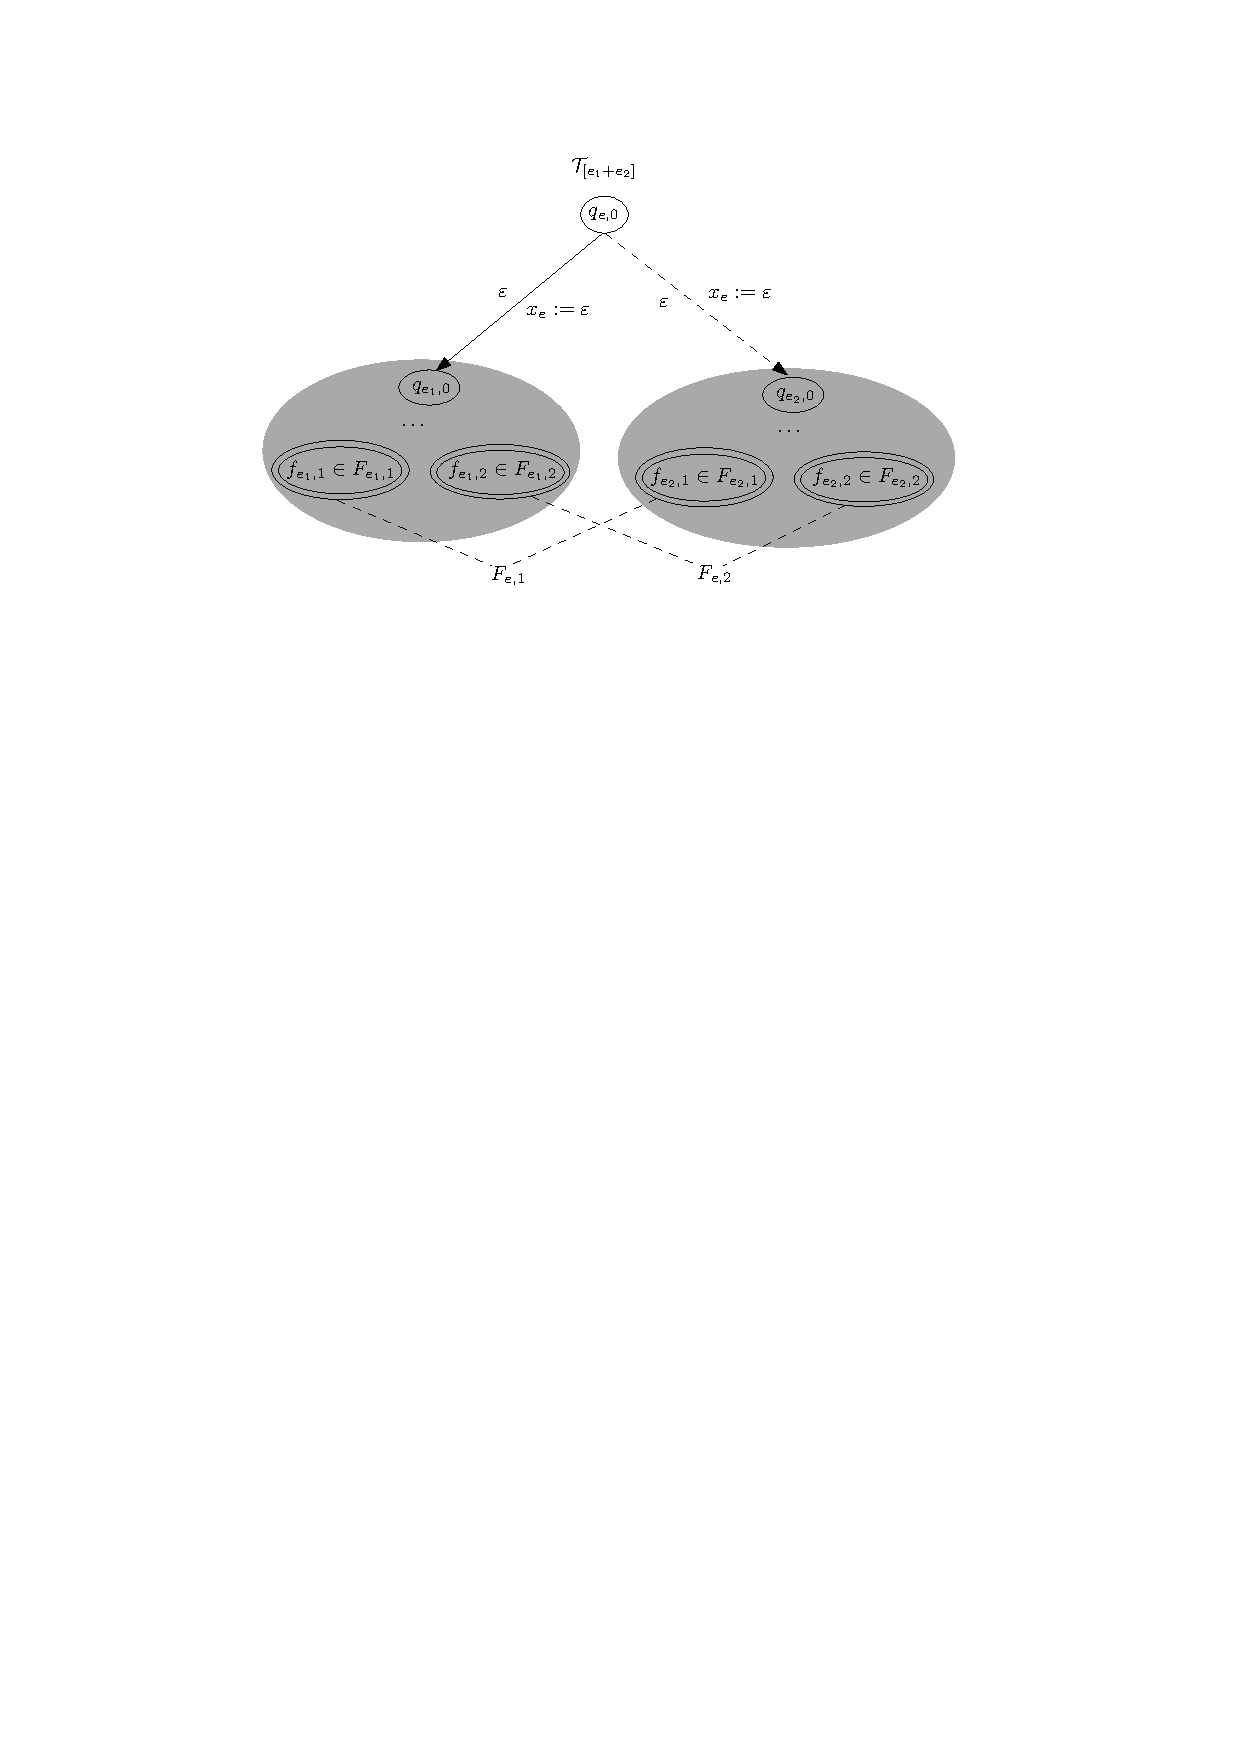
\includegraphics[width = 0.6\textwidth]{reg2pfa-1.pdf}
			\caption{The PFA $\cA_{[e_1+e_2]}$}
			\label{fig-reg2pfa-1}
		\end{figure}  

%%%%%%%%%%%%%%%%%%%%%%%%%%%%%%%%%%%%%%%%%%%%%%%%%%%%%%%%%%%%%%%%%%%%%%%%%%%%%%%%%%%%%%%%%%%%%%%%%%%%%

\paragraph{Case $e = [e_1^?]$} Let $\cA_{e_1} = (Q_{e_1}, \Sigma, X, \delta_{e_1}, \tau_{e_1}, E_1, q_{e_1,0}, (F_{e_1,1}, F_{e_1,2}))$. Then 
\[\cA_e = (Q_{e_1} \cup \{q_{\varepsilon}, q_{e,0}\}, \Sigma, X, 
		\delta_e, \tau_e, E, q_{e,0}, (\{q_{\varepsilon}\}, F_{e_1,2}))\]
where  
		\begin{itemize}
			\item $q_{e,0}  \not \in Q_{e_1}$
			\item $\delta_e(q, a) = \delta_{e_1}(q, a)$ for every $q \in Q_{e_1}$ and $a \in \Sigma$, $\delta_e(q_{e,0}, a)  = ()$ and $\delta_e(q_{\varepsilon}, a) = ()$ for every $a \in \Sigma$, 
			%
			\item $\tau_e(q) = \tau_{e_1}(q)$ for every $q \in Q_{e_1}$, $\tau_e(q_{e,0}) = ((q_{e_1,0},q_{\varepsilon}); ())$,
			\item for each transition $(q, a, q')$ from $\delta_{e_1}$, $E(q,a,q')(x) =E_1(q, a,q')$ and $E(q_{e,0},\varepsilon,q_{\varepsilon})(x) =\varepsilon$
		\end{itemize}
%
Fig.~\ref{fig-reg2pfa-6} depicts the construction.
		\begin{figure}[ht]
			\centering
			%\rule{\linewidth}{0cm}
			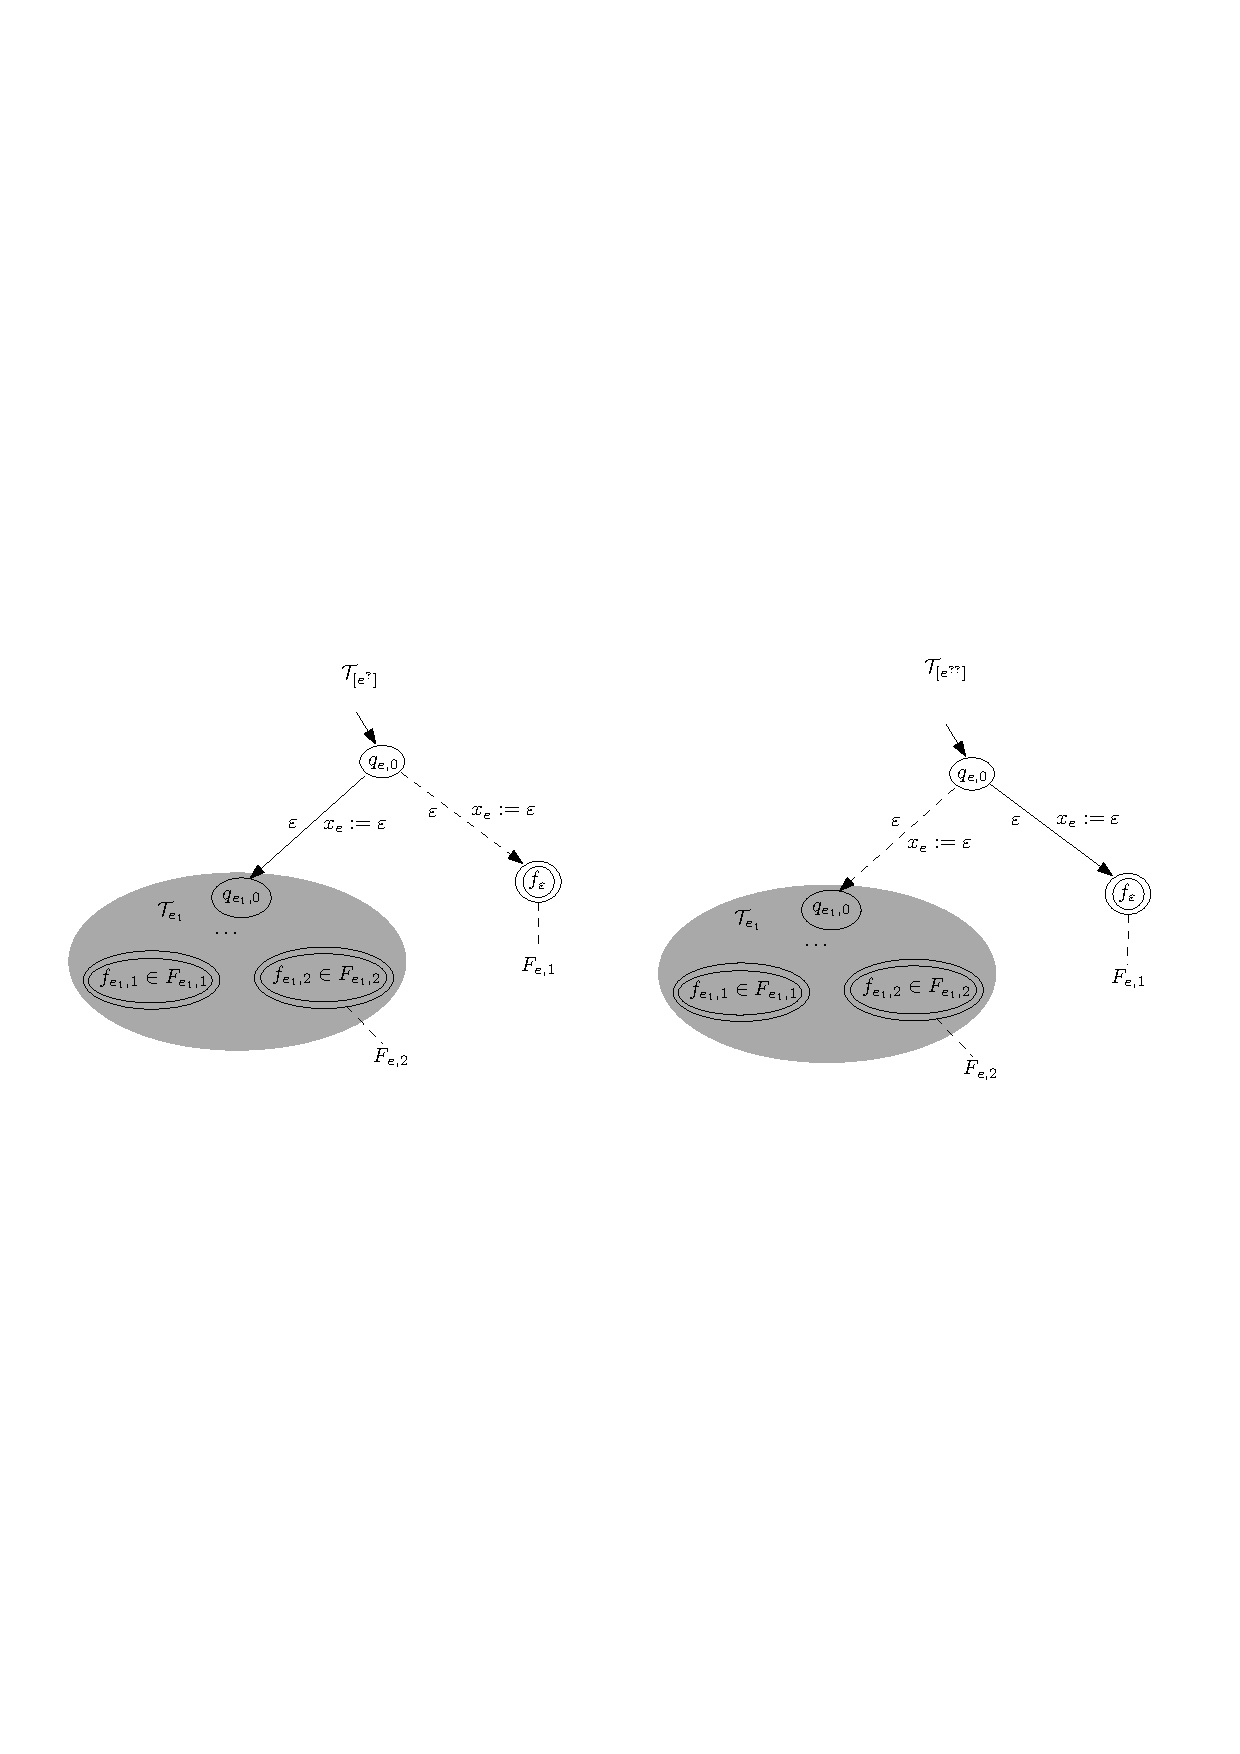
\includegraphics[width = 0.6\textwidth]{reg2pfa-6.pdf}
			\caption{The PFA $\cA_{[e_1^?]}$}
			\label{fig-reg2pfa-6}
		\end{figure}

%%%%%%%%%%%%%%%%%%%%%%%%%%%%%%%%%%%%%%%%%%%%%%%%%%%%%%%%%%%%%%%%%%%%%%%%%%%%%%%%%%%%%%%%%%%%%%%%%%%%%
\paragraph{Case $e = [e_1^{??}]$} 
Let $\cA_{e_1} = (Q_{e_1},
		\Sigma, X, \delta_{e_1}, \tau_{e_1}, E_1 , q_{e_1,0}, (F_{e_1,1}, F_{e_1,2}))$. 
Then 
\[\cA_e = (Q_{e_1} \cup \{q_{e,0}, q_{\varepsilon}\}, \Sigma, X, 
		\delta_e, \tau_e, E, q_{e,0}, (\{q_{\varepsilon}\}, F_{e_1,2}))\] 
where 
		\begin{itemize}
			\item $q_{e,0}  \not \in Q_{e_1}$
			\item $\delta_e(q, a) = \delta_{e_1}(q, a)$ for every $q \in Q_{e_1}$ and $a \in \Sigma$, $\delta_e(q_{e,0}, a)  = ()$ and $\delta_e(q_{\varepsilon}, a) = ()$ for every $a \in \Sigma$, 
			%
			\item $\tau_e(q) = \tau_{e_1}(q)$ for every $q \in Q_{e_1}$, $\tau_e(q_{e,0}) = ((q_{\varepsilon}, q_{e_1,0}); ())$,
			
			\item for each transition $(q, a, q')$ from $\delta_{e_1}$, $E(q,a,q')(x) = E_1(q,a,q')(x)$ and $E(q_{e,0},\varepsilon,q_{\varepsilon})(x) =\varepsilon$
		\end{itemize}
Fig.~\ref{fig-reg2pfa-7} depicts the construction. 
		\begin{figure}[ht]
			\centering
			%\rule{\linewidth}{0cm}
			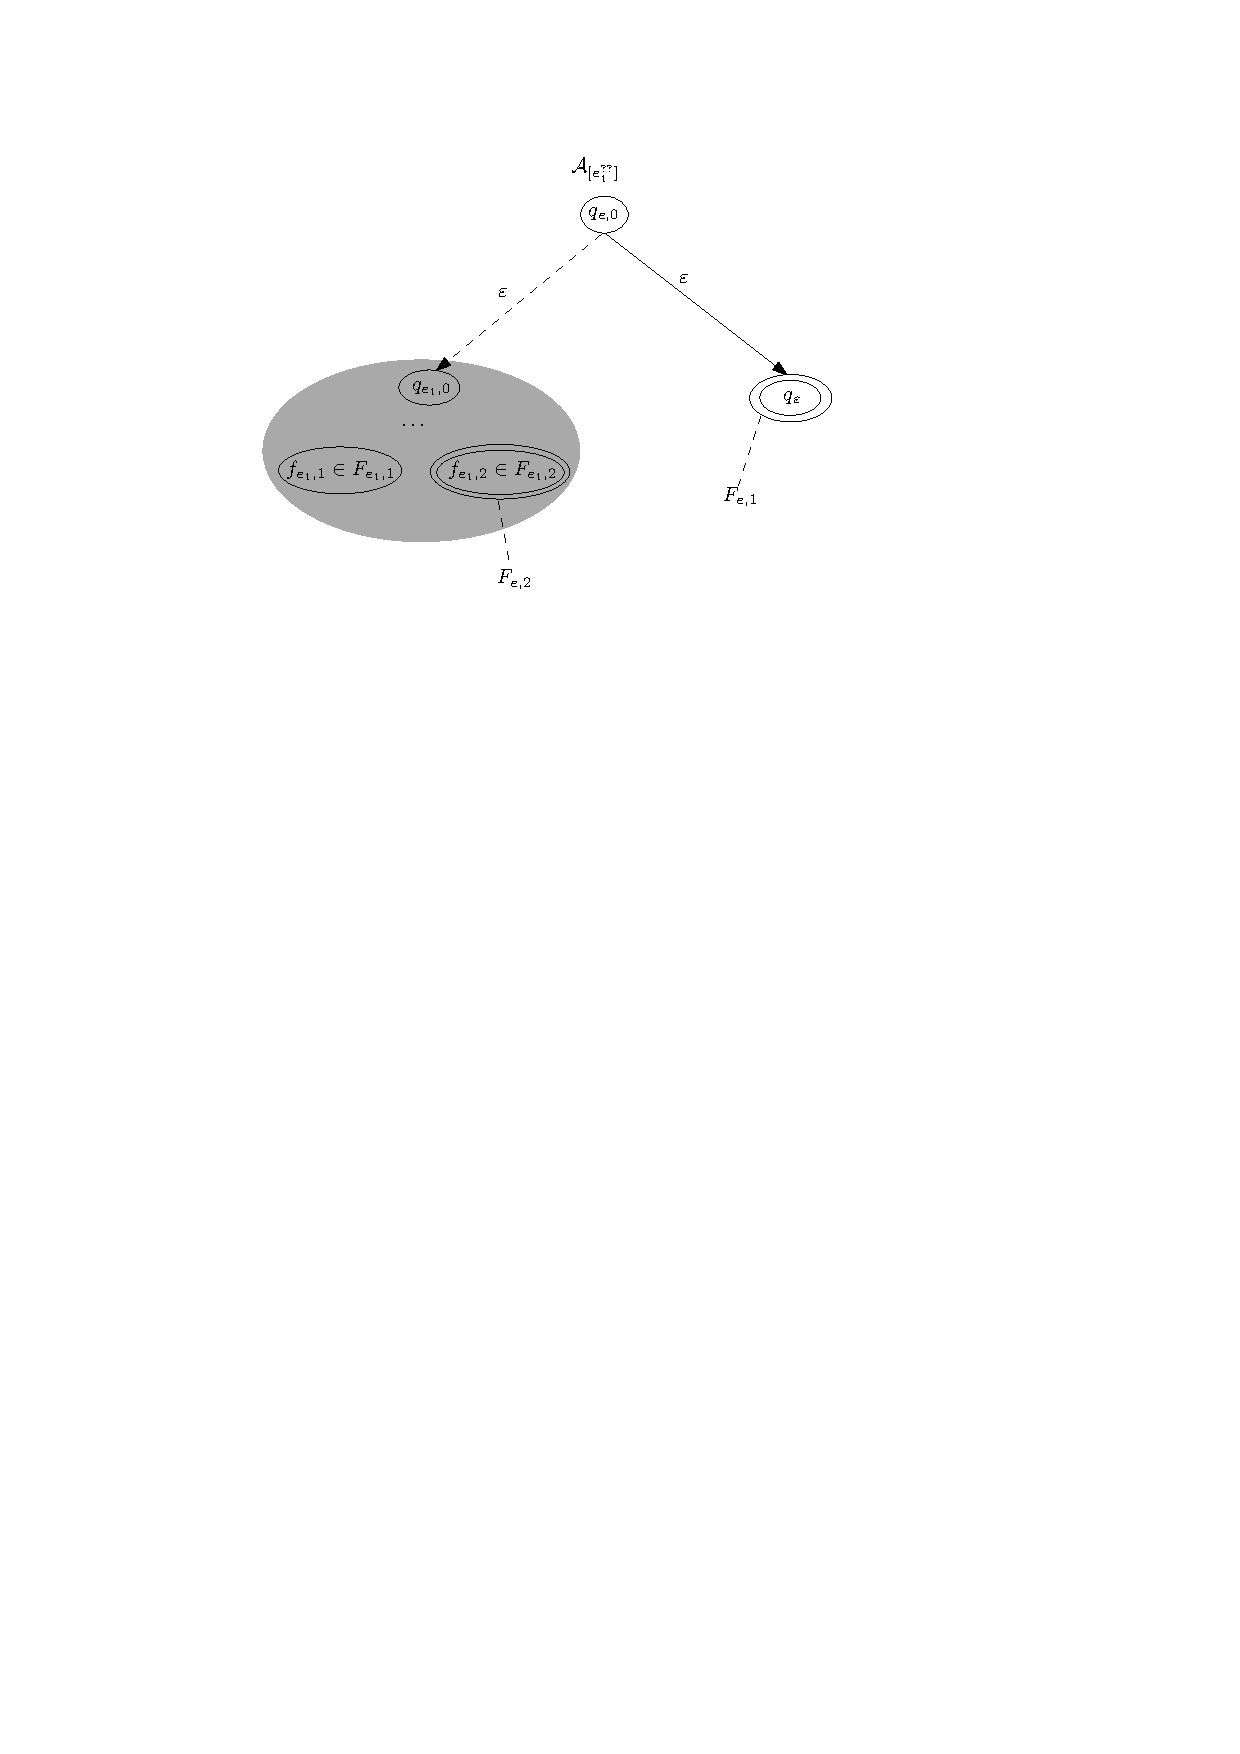
\includegraphics[width = 0.5\textwidth]{reg2pfa-7.pdf}
			\caption{The PFA $\cA_{[e_1^{??}]}$}
			\label{fig-reg2pfa-7}
		\end{figure}
	
%%%%%%%%%%%%%%%%%%%%%%%%%%%%%%%%%%%%%%%%%%%%%%%%%%%%%%%%%%%%%%%%%%%%%%%%%%%%%%%%%%%%%%%%%%%%%%%%%%%%%
\paragraph{Case $e = [e_1 \concat e_2]$} 
Let 
\[\cA_{e_1} = (Q_{e_1}, \Sigma, X_1, \delta_{e_1}, \tau_{e_1}, E_1, q_{e_1,0}, (F_{e_1,1}, F_{e_1,2}))\]
%
\[\cA_{e_2} = (Q_{e_2}, \Sigma, X_2, \delta_{e_2}, \tau_{e_2}, E_2, q_{e_2,0}, (F_{e_2, 1}, F_{e_2,2}))\] and
%
$\cA'_{e_2} = (Q'_{e_2}, \Sigma, X_2, \delta'_{e_2}, \tau'_{e_2}, E_2', q'_{e_2,0}, (F'_{e_2, 1}, F'_{e_2,2}))$ be a fresh copy of $\cA_{e_2}$. We assume that $X_1\cap X_2=\emptyset$. Then 
%
\[\cA_e = ( Q_{e_1} \cup Q_{e_2} \cup Q'_{e_2}, \Sigma, X_1\cup X_2, \delta_e, \tau_e, q_{e_1,0}, (F_{e_2,1}, F_{e_2,2} \cup F'_{e_2,1} \cup F'_{e_2,2}))\] where 
	\begin{itemize}
	 \item for every $i \in \{1,2\}$, $q \in Q_{e_i}$ and $a \in \Sigma$, $\delta_e(q, a) = \delta_{e_i}(q, a)$,
			%
	\item for every $q' \in Q'_{e_2}$ and $a \in \Sigma$, $\delta_e(q', a) = \delta'_{e_2}(q',a)$, 
			%    
	\item for every $q \in Q_{e_2}$, $\tau_e(q) = \tau_{e_2}(q)$ and $\tau_e(q') = \tau'_{e_2}(q')$, 
			%
	\item for every $q \in Q_{e_1} \setminus (F_{e_1,1} \cup F_{e_1,2})$, $\tau_e(q) = \tau_{e_1}(q)$, for every $f_{e_1,1} \in F_{e_1,1}$, $\tau_e(f_{e_1,1}) = ((q_{e_2,0}); ())$, and for every $f_{e_1,2} \in F_{e_1,2}$, $\tau_e(f_{e_1,2}) = ((q'_{e_2,0}), ())$,
	%
	\item for $i\in \{1,2\}$ and each transition $(q, a, q')$ from $\delta_{e_i}$, $E(q,a,q')(x) = E_i(q,a,q')(x)$ for $x\in X_i$; for $x\in X_2$, $E(f_{e_1,1},\varepsilon,q_{e_2,0})(x) =\varepsilon$, $E(f_{e_1,2},\varepsilon,q'_{e_2,0})(x) =\varepsilon$.
  \end{itemize}
 Fig.~\ref{fig-reg2pfa-2} depicts the construction. 
		\begin{figure}[ht]
			\centering
			%\rule{\linewidth}{0cm}
			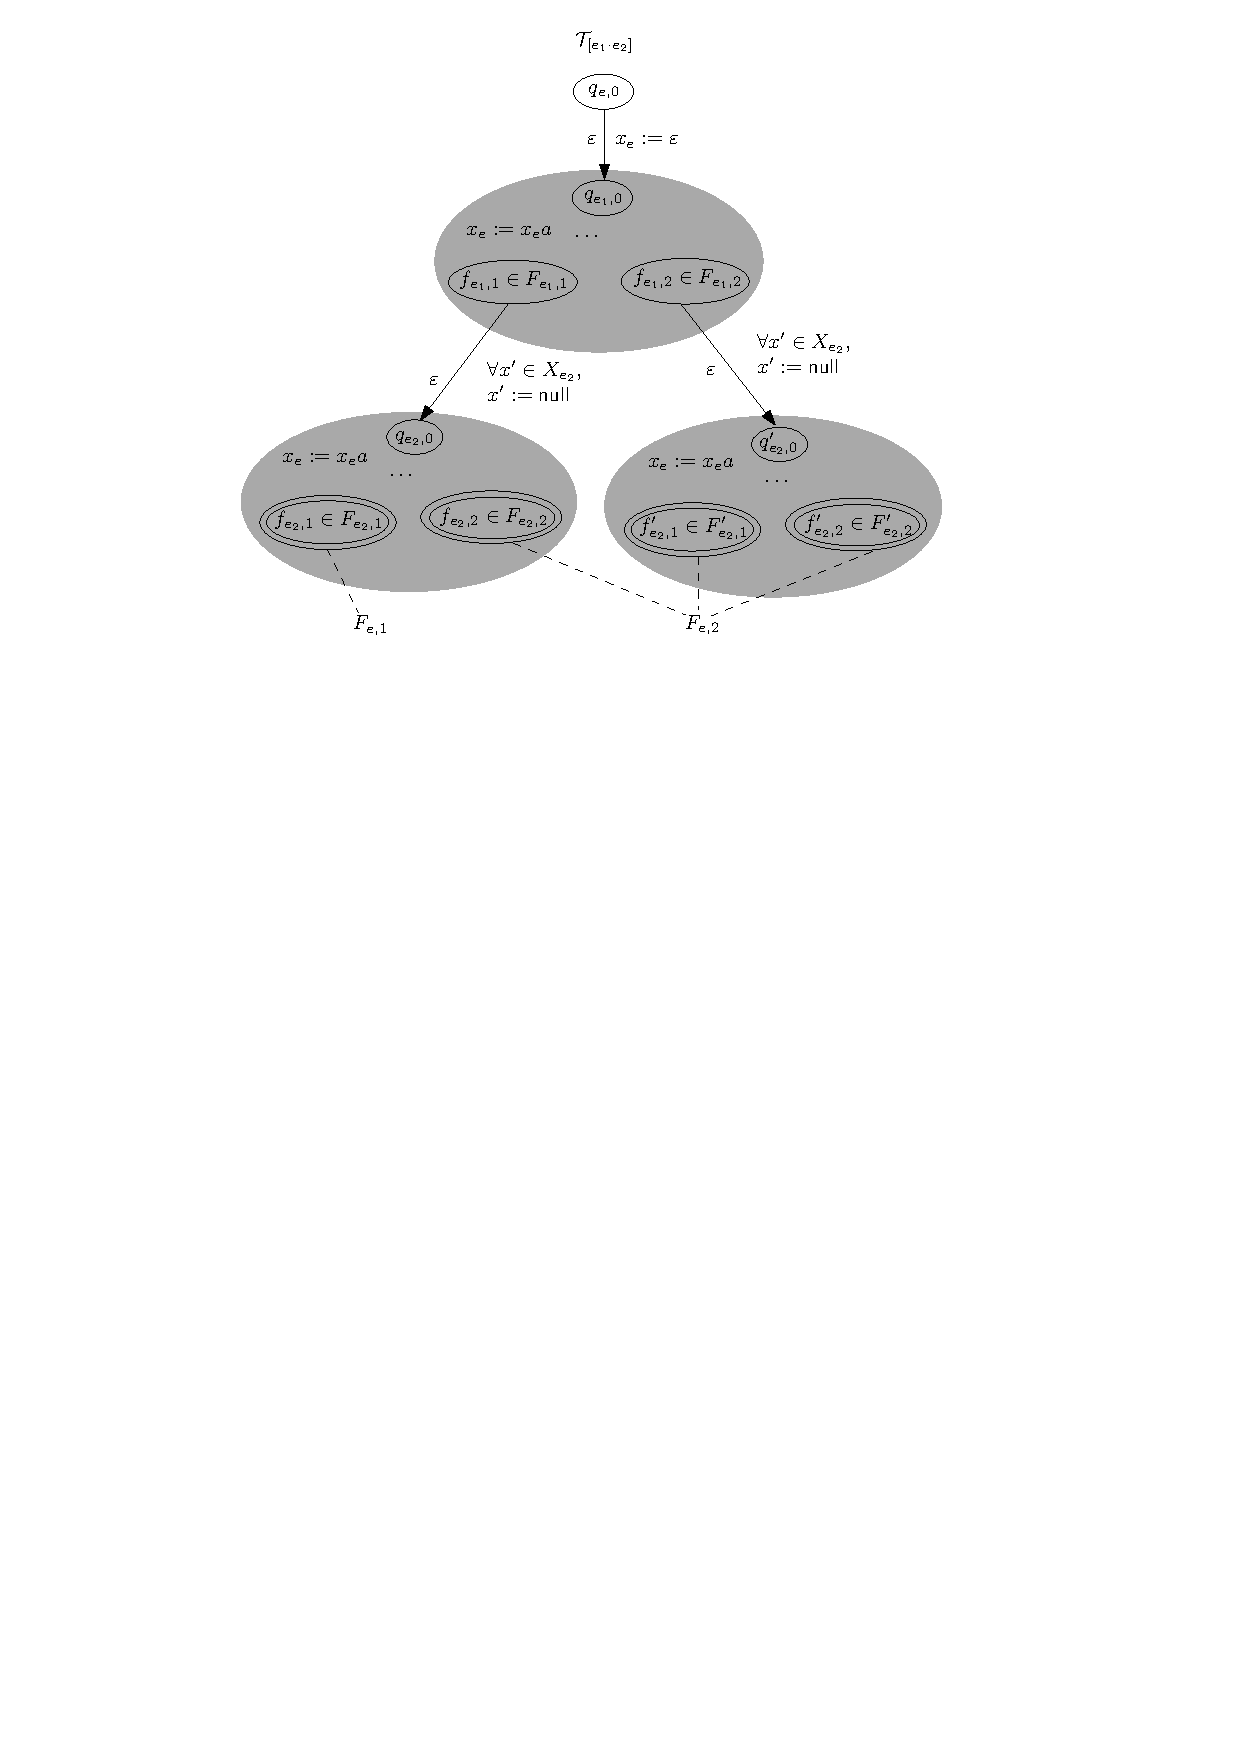
\includegraphics[width = 0.6\textwidth]{reg2pfa-2.pdf}
			\caption{The PFA $\cA_{[e_1\concat e_2]}$}
			\label{fig-reg2pfa-2}
		\end{figure}  
	

%%%%%%%%%%%%%%%%%%%%%%%%%%%%%%%%%%%%%%%%%%%%%%%%%%%%%%%%%%%%%%%%%%%%%%%%%%%%%%%%%%%%%%%%%%%%%%%%%%%%%

\paragraph{Case $e = [e_1^{\ast}]$} 
Let $\cA_{e_1} = (Q_{e_1}, \Sigma, X_1, \delta_{e_1}, \tau_{e_1}, E_1, q_{e_1,0}, (F_{e_1,1}, F_{e_1,2}))$. Then
\[ \cA_e = (Q_{e_1} \cup \{q_{e,0}, f_{e,0}, f_{e,1}\}, \Sigma, X_1, \delta_e, E, \tau_e, q_{e,0}, (\{f_{e,0}\}, \{f_{e,1}\}))\] where 
		\begin{itemize}
			\item $q_{e,0}, f_{e,0} \not \in Q_{e_1}$,
			
			\item for every $q \in Q_{e_1}$ and $a \in \Sigma$, $\delta_e(q, a) = \delta_{e_1}(q, a)$, 
			%moreover, $\delta(q_0, a) = \delta(f_0, a)  = ()$,
			
			\item for every $q \in Q_{e_1} \setminus (F_{e_1,1} \cup F_{e_1,2})$,  $\tau_e(q) = \tau_{e_1}(q)$, moreover, $\tau_e(q_{e,0}) = ((q_{e_1,0},f_{e,0}); ())$,  $\tau_e(q) = ((q_{e_1,0});())$ for every $q \in F_{e_1,1}$, $\tau_e(q) = ((q_{e_1,0}, f_{e,1});())$ for every $q \in F_{e_1,2}$, $\tau_e(f_{e,0}) =\tau_e(f_{e,1}) = (();())$. (Intuitively, the $\varepsilon$-transitions from $q_{e,0}$ to $q_{e_1,0}$ and $f_{e,0}$, from each $q \in F_{e_1,1}$ to $q_{e_1,0}$, and from $q \in F_{e_1,2}$ to $q_{e_1,0}$ and $f_{e,1}$ respectively are added, moreover, the $\varepsilon$-transition from $q_{e,0}$ to $f_{e,0}$ and from $q \in F_{e_1,2}$ to $f_{e,1}$ are of the lowest priority.)
			
			\item for each transition $(q, a, q')$ from $\delta_{e_1}$, $E(q,a,q')(x) = E_1(q,a,q')(x)$, and $E(q_{e,0},\varepsilon,q_{f_e,0})(x) =\varepsilon$, $E(q_{e,0},\varepsilon,q_{e_1,0})(x) =\varepsilon$, $E(f_{e_1,2},\varepsilon,f_{e,1})(x) =x$.
		\end{itemize}

%%%%%%%%%%%%%%%%%%%%%%%%%%%%%%%%%%%%%%%%%%%%%%%%%%%%%%%%%%%%%%%%%%%%%%%%%%%%%%%%%%%%%%%%%%%%%%%%%%%%%
\paragraph{Case $e = [e_1^{+}]$} Then $\cA_e$ is constructed as $\cA_{[e_1 \concat [e^\ast_1]]}$.
		
%%%%%%%%%%%%%%%%%%%%%%%%%%%%%%%%%%%%%%%%%%%%%%%%%%%%%%%%%%%%%%%%%%%%%%%%%%%%%%%%%%%%%%%%%%%%%%%%%%%%%
\paragraph{Case $e = [e_1^{\ast?}]$} Let $\cA_{e_1} = (Q_{e_1}, \Sigma, X_1, \delta_{e_1}, \tau_{e_1}, E_1, q_{e_1,0}, (F_{e_1,1}, F_{e_1,2}))$. 
Then 
\[\cA_e = (Q_{e_1} \cup \{q_{e,0}, f_{e,0}, f_{e,1}\}, \Sigma, X_1, \delta_e, \tau_e, E, q_{e,0}, (\{f_{e,0}\}, \{f_{e,1}\}))\]  
where 
		\begin{itemize}
			\item $q_{e,0}, f_{e,0} \not \in Q_{e_1}$,
			
			\item for every $q \in Q_{e_1}$ and $a \in \Sigma$, $\delta_e(q, a) = \delta_{e_1}(q, a)$, 
			%moreover, $\delta(q_0, a) = \delta(f_0, a)  = ()$,
			
			\item for every $q \in Q_{e_1} \setminus (F_{e_1,1} \cup F_{e_1,2})$,  $\tau_e(q) = \tau_{e_1}(q)$, moreover, $\tau_e(q_{e,0}) = ((f_{e,0}, q_{e_1,0}); ())$,  $\tau_e(q) = ((q_{e_1,0});())$ for every $q \in F_{e_1,1}$, $\tau_e(q) = ((f_{e,1}, q_{e_1,0});())$ for every $q \in F_{e_1,2}$, $\tau_e(f_{e,0}) =\tau_e(f_{e,1}) = (();())$. (Intuitively, the $\varepsilon$-transitions from $q_{e,0}$ to $f_{e,0}$ and $q_{e_1,0}$ , from each $q \in F_{e_1,1}$ to  $q_{e_1,0}$, and from each $q \in F_{e_1,2}$ to $f_{e,1}$ and $q_{e_1,0}$ respectively are added, moreover, the $\varepsilon$-transition from $q_{e,0}$ to $q_{e_1,0}$ and from $q \in F_{e_1,2}$ to $q_{e_1,0}$ are of the lowest priority.)
			
			\item for each transition $(q, a, q')$ from $\delta_{e_1}$, $E(q,a,q')(x) = E_1(q,a,q')(x)$, and $E(q_{e,0},\varepsilon,q_{f_e,0})(x) =\varepsilon$, $E(q_{e,0},\varepsilon,q_{e_1,0})(x) =\varepsilon$, $E(f_{e_1,2},\varepsilon,f_{e,1})(x) =x$.
		\end{itemize}

 
%%%%%%%%%%%%%%%%%%%%%%%%%%%%%%%%%%%%%%%%%%%%%%%%%%%%%%%%%%%%%%%%%%%%%%%%%%%%%%%%%%%%%%%%%%%%%%%%%%%%%
\paragraph{Case $e = [e_1^{+?}]$} then $\cA_e$ is constructed as $\cA_{[e_1 \concat [e_1^{*?}]]}$.

Fig.~\ref{fig-reg2pfa-3} depicts the construction. 
\begin{figure}[ht]
	\centering
	%\rule{\linewidth}{0cm}
	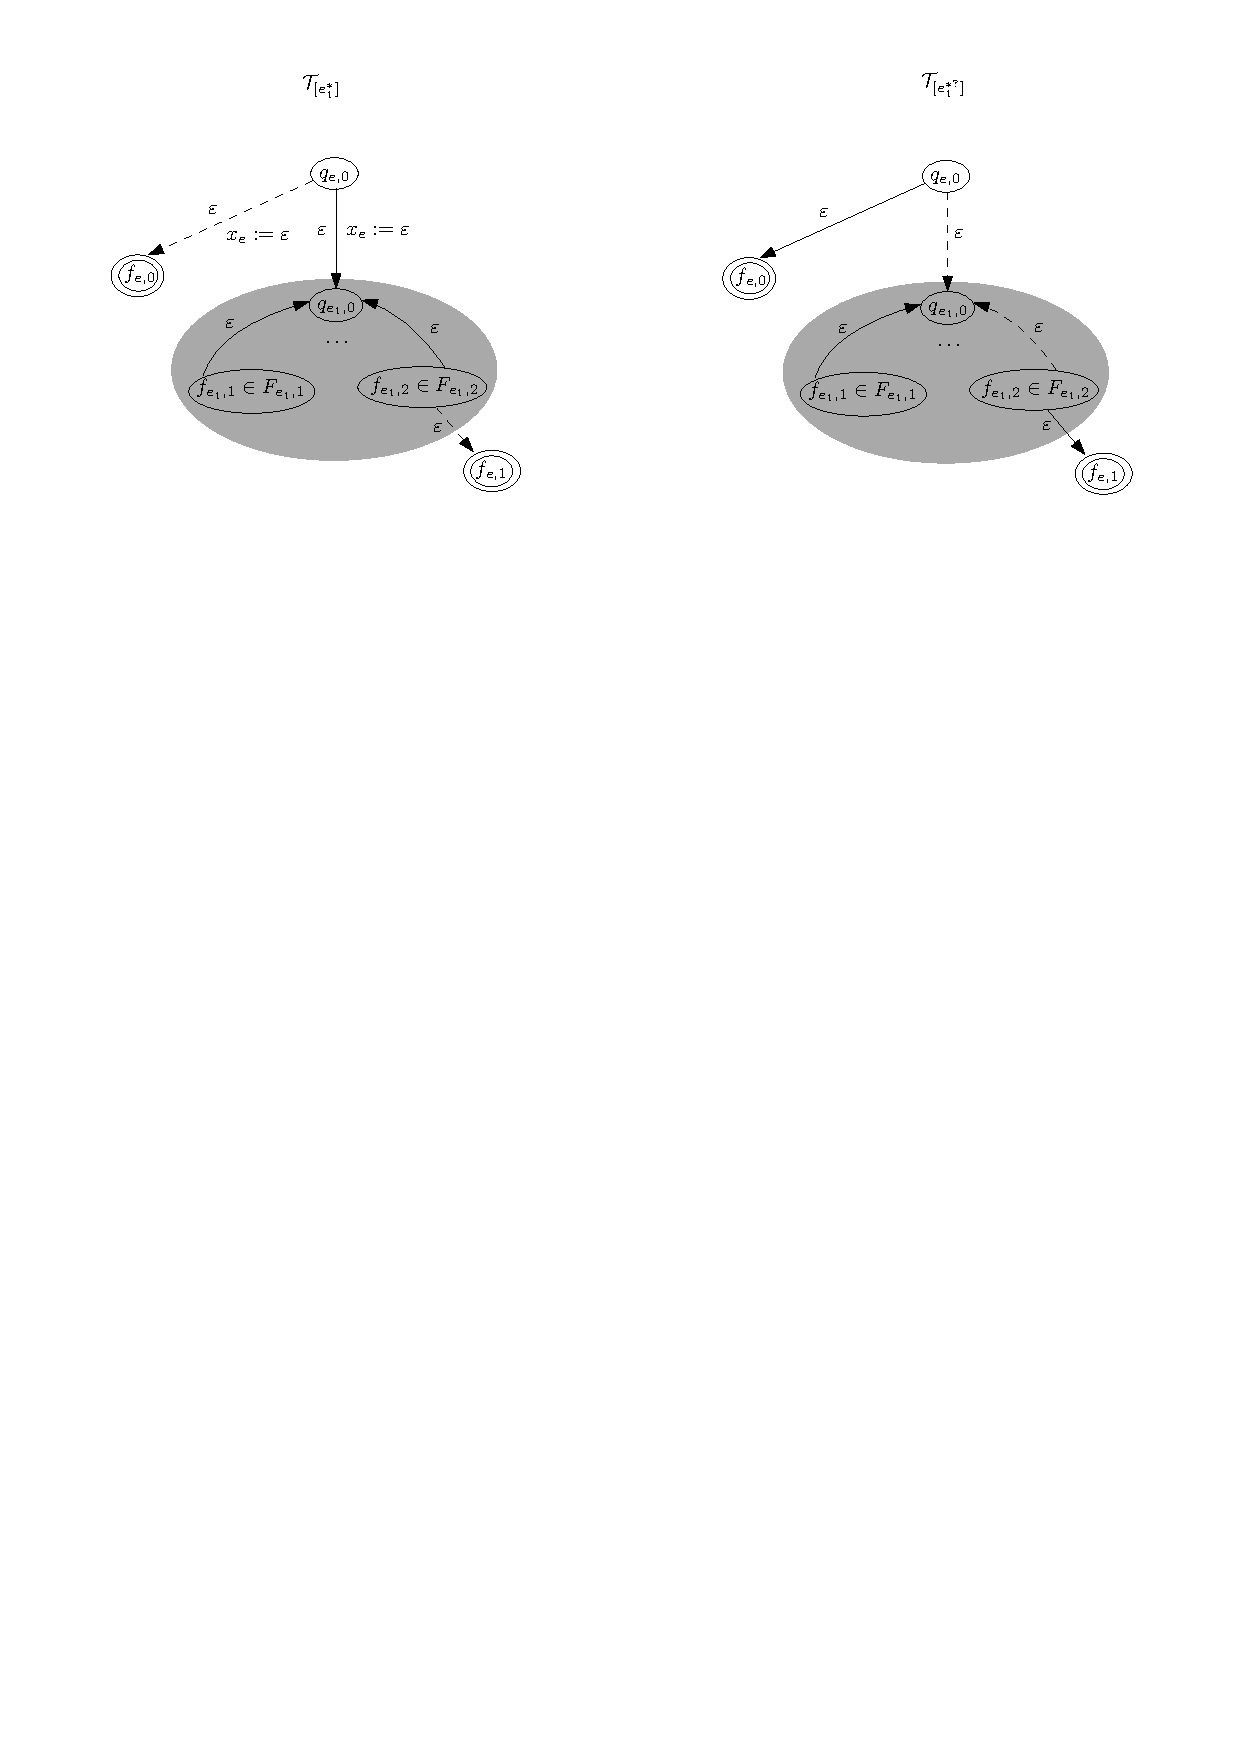
\includegraphics[width = 0.8\textwidth]{reg2pfa-3.pdf}
	\caption{The PFA $\cA_{[e_1^\ast]}$ and $\cA_{[e_1^{\ast?}]}$}
	\label{fig-reg2pfa-3}
\end{figure}

%%%%%%%%%%%%%%%%%%%%%%%%%%%%%%%%%%%%%%%%%%%%%%%%%%%%%%%%%%%%%%%%%%%%%%%%%%%%%%%%%%%%%%%%%%%%%%%%%%%%%
\paragraph{Case $e = [e_1^{\{m_1,m_2\}}]$} Then $\cA_e$ is constructed as the concatenation of $\cA_{e_1^{m_1}}$ and $\cA^\prime_{e_1^{\{1,m_2-m_1\}}}$, where $\cA_{e_1^{m_1}}$ is the PFA corresponding to consecutive concatenations of $m_1$ copies of $e_1$, and $\cA^\prime_{e_1^{\{1,m_2-m_1\}}}$ is illustrated in Fig.~\ref{fig-reg2pfa-4}, which consists of $m_2-m_1$ copies of $\cA_{e_1}$, say $(\cA^{(i)}_{e_1})_{i \in [m_2-m_1]}$, as well as the $\varepsilon$-transition from $q^{(1)}_{e_1,0}$ to a fresh state $f^\prime_0$ (of the lowest priority), and the $\varepsilon$-transitions from each $f^{(i)}_{e_1,2} \in F^{(i)}_{e_1,2}$ to $q^{(i+1)}_{e_1,0}$ (of the highest priority), and a fresh state $f^\prime_1$ (of the lowest priority). The accepting states of $\cA^\prime_{e_1^{\{1,m_2-m_1\}}}$ are $(\{f_0'\},\{f_1'\})$. (Intuitively, each $\cA^{(i)}_{e_1}$ accepts only nonempty strings, thus $f^{(i)}_{e_1,1} \in F^{(i)}_{e_1,1}$ contains no outgoing transitions in $\cA^\prime_{e_1^{\{1,m_2-m_1\}}}$. )
		%
		\begin{figure}[ht]
			\centering
			%\rule{\linewidth}{0cm}
			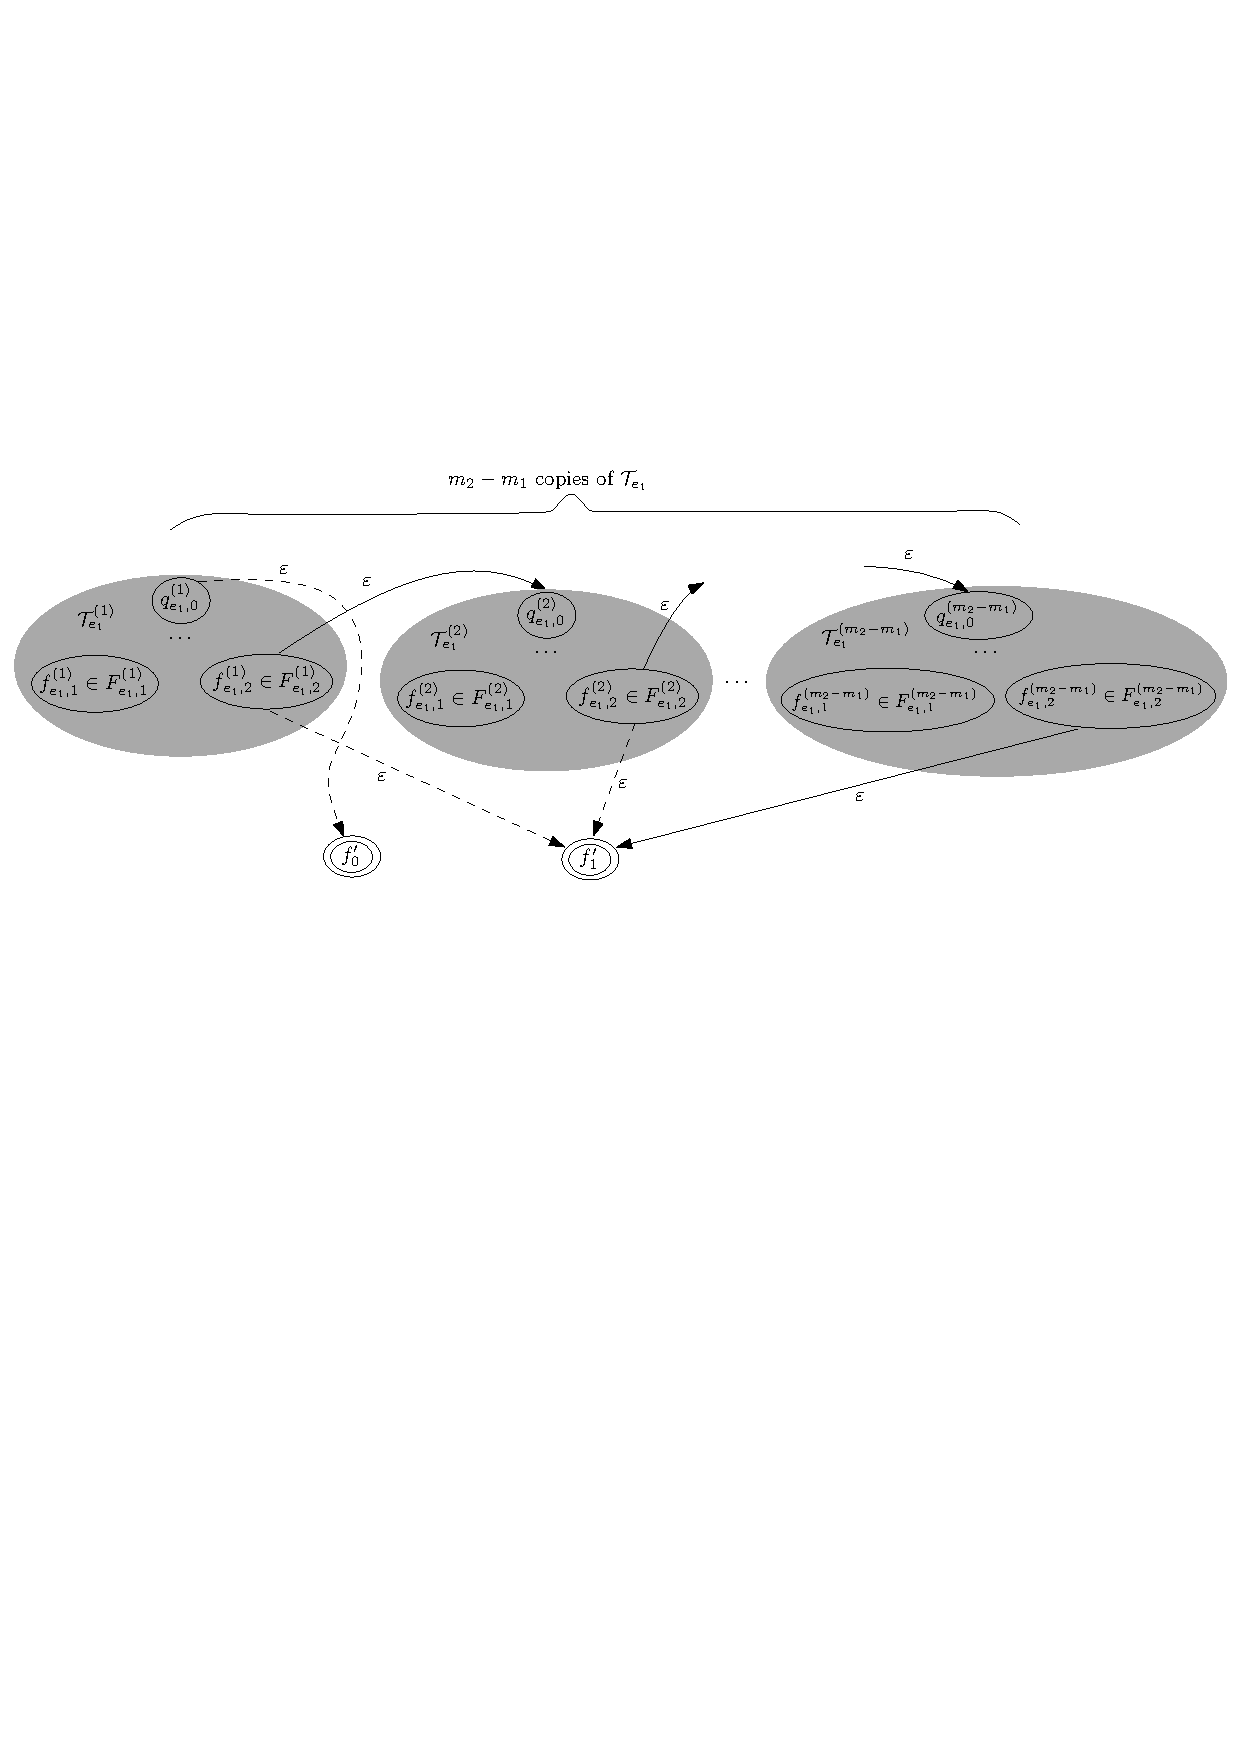
\includegraphics[width = 0.8\textwidth]{reg2pfa-4.pdf}
			\caption{The PFA $\cA^\prime_{e_1^{\{1,m_2-m_1\}}}$}
			\label{fig-reg2pfa-4}
		\end{figure}  


%%%%%%%%%%%%%%%%%%%%%%%%%%%%%%%%%%%%%%%%%%%%%%%%%%%%%%%%%%%%%%%%%%%%%%%%%%%%%%%%%%%%%%%%%%%%%%%%%%%%%
\paragraph{Case $e = [e_1^{\{m_1,m_2\}?}]$} Then $\cA_e$ is constructed as the concatenation of $\cA_{e_1^{m_1}}$ and $\cA^\prime_{e_1^{\{1,m_2-m_1\}?}}$, where $\cA^\prime_{e_1^{\{1,m_2-m_1\}?}}$ is illustrated in Fig.~\ref{fig-reg2pfa-5}, which is the same as $\cA^\prime_{e_1^{\{1,m_2-m_1\}}}$ in Fig.~\ref{fig-reg2pfa-4}, except that the priorities of $\varepsilon$-transition from $q^{(1)}_{e_1,0}$ to $f^\prime_0$ has the highest priority and  the priorities of $\varepsilon$-transitions from each $f^{(i)}_{e_1,2} \in F^{(i)}_{e_1,2}$ to $f^\prime_1$ are reversed.
		\begin{figure}[ht]
			\centering
			%\rule{\linewidth}{0cm}
			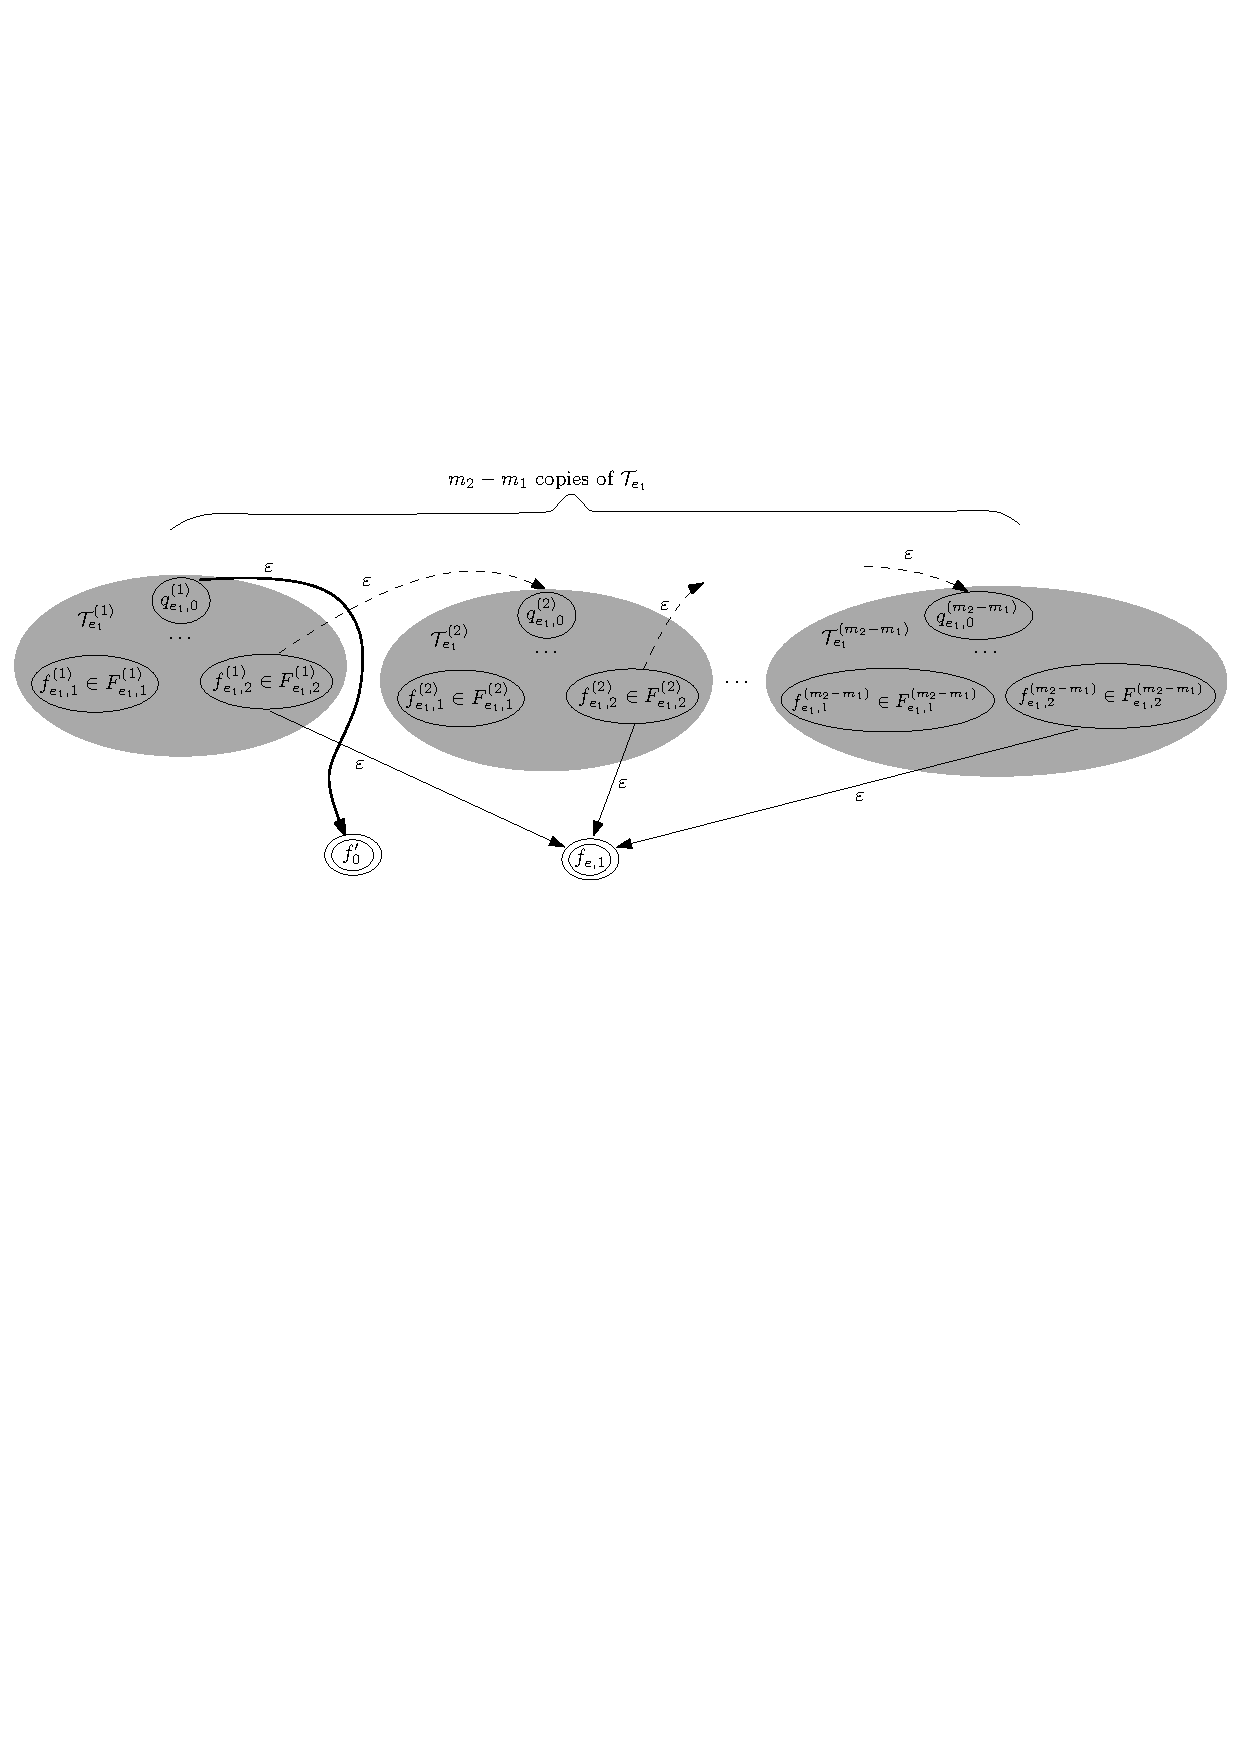
\includegraphics[width = 0.8\textwidth]{reg2pfa-5.pdf}
			\caption{The PFA $\cA^\prime_{e_1^{\{1,m_2-m_1\}?}}$}
			\label{fig-reg2pfa-5}
		\end{figure}  
%%%%%%%%%%%%%%%%%%%%%%%%%%%%%%%%%%%%%%%%%%%%%%%%%%%%%%%%%%%%%%%%%%%%%%%%%%%%%%%%%%%%%%%%%%%%%%%%%%%%%%%%

 %can be constructed 
%(in linear time)

% such that 
%	\begin{itemize}
%		\item $\cA_e$ has a unique initial state without incoming transitions and a unique final state without outgoing transitions,
%		%
%		\item for subexpression $e'$ of $e$, $\cA_e$ contains at least one isomorphic copy of $\cA_{e'}$ (i.e. the PFA constructed for $e'$), denoted by ${\sf Sub}_{e'}[\cA_e]$. 
%	\end{itemize}

%Let us use ${\sf Sub}_{e'}[\cA_e]$ to denote the isomorphic copy of $\cA_{e'}$ in $\cA_e$, as mentioned in Proposition~\ref{prop-rwre-to-pfa}.

%\begin{proof}
%	For any $e \in \cgexp$, a PFA $\cA_e$ is constructed recursively in the sequel. The constructed PFA $\cA_e$ satisfies that 
%	\begin{itemize}
%		\item it has a unique initial state without incoming transitions and each of its final states has no outgoing transitions,
%		\item all the transitions out of the initial state are $\varepsilon$-transitions, 
%		\item the set of final states is divided into two disjoint subsets $F_1, F_2$ such that for each $w \in \Sigma^*$ satisfying that $q_0 \xrightarrow[\cA_e]{w} q$ for some $q \in F_1$ (resp. $q \in F_2$), $w = \varepsilon$ (resp. $w \neq \varepsilon$).
%	\end{itemize}



\begin{example}\label{exmp-pfa}
	The PFA corresponding to the RWRE $e = [[([\Gamma^+])\concat .?] \concat ([\Gamma^*])]$ 
	%in Example~\ref{exmp-regex-match-tree}
	%
	is illustrated in Fig.~\ref{fig-pfa}, where the dashed (resp. thicker solid) lines represent the $\varepsilon$-transitions of lower (resp. higher) priorities than non-$\varepsilon$ transitions (if there is any), and the doubly circled states are final states. For instance, $\delta(q_1, \ell) = (q_1)$ for every $\ell \in \{0, \dots, 9\}$, $\delta(q_1, .) = ()$, $\tau(q_1) = ((); (q_2))$. Since the $\varepsilon$-transition has lower priority than the $\ell$-transition at the state $q_1$, whenever the currently scanned letter is $\ell \in \{0,\cdots,9\}$ at $q_1$,  the PFA will choose to go to $q_1$ greedily, until there is no more $\ell  \in \{0,\cdots,9\}$. (In this case, it has to choose the $\epsilon$-transition and goes to $q_2$.)
	%
	\begin{figure}[ht]
		
		\centering
		%\rule{\linewidth}{0cm}
		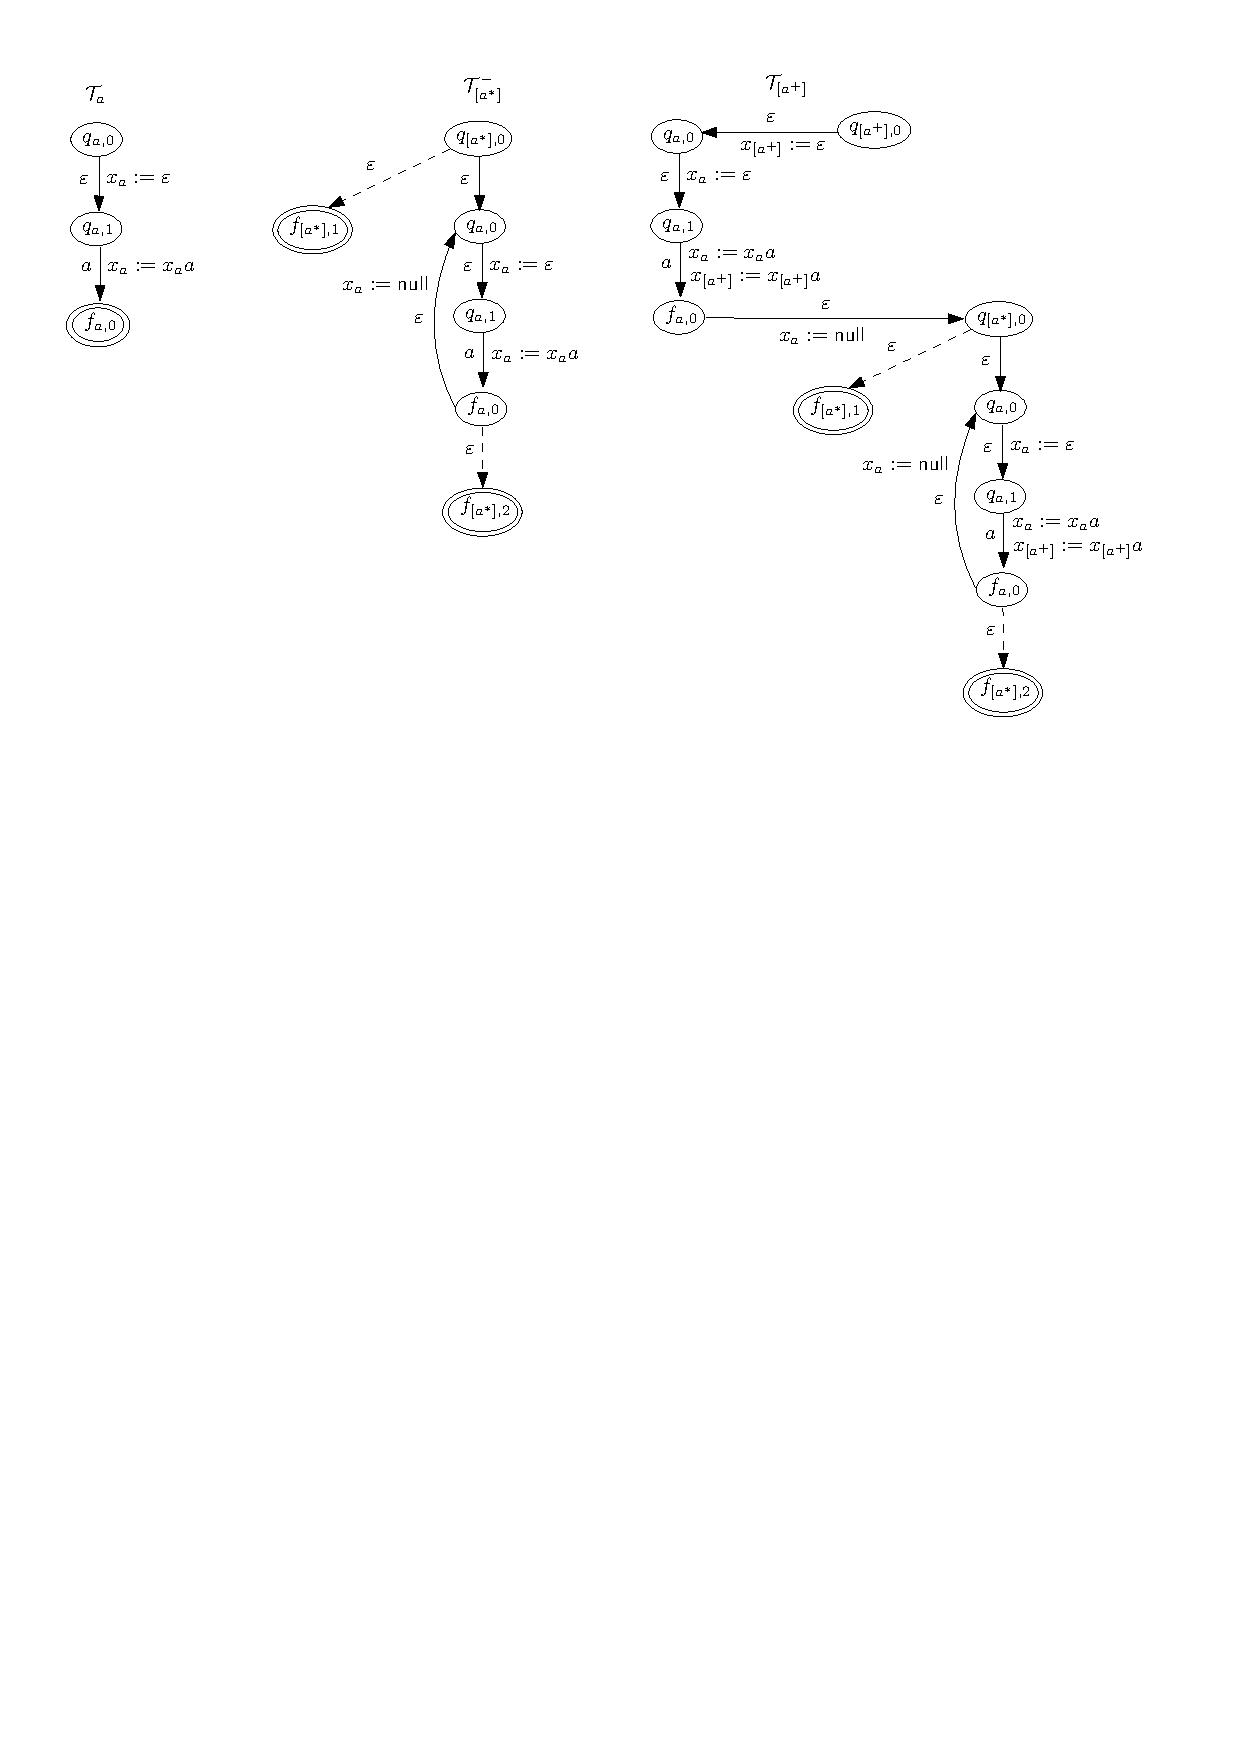
\includegraphics[width=0.9\textwidth]{pfa-new.pdf}
		\caption{The PFA for $e = [[([\Gamma^+])\concat .?] \concat ([\Gamma^*])]$, where $\Gamma = \{0, \cdots, 9\}$}
		\label{fig-pfa}
		
	\end{figure}
\end{example}



%%%%%%%%%%%%%%%%%%%%%%%%%%%%%%%%%%%%%%%%%%
\subsection{Validation experiments for the formal semantics} \label{sect:valid}

%!TEX root = main.tex
\paragraph{Validation experiments for the formal semantics} \label{sect:valid}
We have defined %the formal semantics of the regular-expression 
{\regexp}-string matching by constructing {\PSST}s. %out of regular expressions. 
In the sequel, we conduct experiments to validate the formal semantics against the actual JavaScript {\regexp}-string matching.

Let $\opset$ denote the set of {\regexp} operators: alternation $+$, concatenation $\concat$, optional $?$, lazy optional $??$, Kleene star $*$, lazy Kleene star $*?$, Kleene plus $+$, lazy Kleene plus $+?$, repetition $\{m_1,m_2\}$, and lazy repetition $\{m_1,m_2\}?$. Moreover, let $\opset^{2}$ (resp. $\opset^{3}$) denote the set of pairs (resp. triples) of operators from $\opset$. 
Aiming at a good coverage of different syntactical ingredients of {\regexp}, we generate regular expressions for every element of $\opset^{\le 3} = \opset \cup \opset^2 \cup \opset^3$.
As arguments of these operators, we consider the following character sets: $\mathbb{S} = \{$a, $\ldots$, z$\}$, $\mathbb{C}=\{$A, $\ldots$, Z$\}$, $\mathbb{D} = \{0,\ldots,9\}$, and $\mathbb{O}$, the set of ASCII symbols not belonging to $\mathbb{S} \cup \mathbb{C} \cup \mathbb{D}$.
Intuitively, these character sets correspond to JavaScript character classes [a-z], [A-Z], [0-9], and [{\textasciicircum}a-zA-Z0-9] (where {\textasciicircum} denotes complement).
Moreover, for the regular expression generated for each element of $\opset^{\le 3}$, we set the subexpression corresponding to its first component as the capturing group. 
For instance, for the pair $(*?, *)$, we generate the {\regexp} $[([\mathbb{S}^*?])^{*}]$. In the end, we generate $10+10*10+10*10*10 = 1110$ {\regexp}s. 

For each generated {\regexp} $e$, we construct a PSST $\psst_e$, whose output corresponds to the matching of the first capturing group in $e$.  Moreover, we generate from $\psst_e$ an input string $w$ as well as the corresponding output $w'$. We require that the length of $w$ is no less than some threshold (e.g., $10$), in order to avoid the empty string and facilitate a  meaningful comparison with the actual semantics of JavaScript regular-expression matching. 
Let {\sf reg} be the JavaScript regular expression corresponding to $e$. Then we execute the following JavaScript program $\cP_{e,w}$,
\begin{center}
{
\small
\begin{minted}{javascript}
      var x = w; console.log(x.match(reg)[1]);
\end{minted}
}
\end{center}
and confirm that its output is equal to $w'$, thus validating that the formal semantics of  \regexp-string matching defined by PSSTs is consistent with the actual semantics of JavaScript {\sf match} function. For instance, for the {\regexp} expression $[([\mathbb{S}^*?])^{*}]$, we generate from the $\psst_e$ the input string $w= aaaaaaaaaa$, together with the output $a$. Then we generate  the JavaScript program from ${\sf reg}$ and $w$, execute it, and obtain the same output $a$.

In all the generated {\regexp}s, we confirm the consistency of the formal semantics of  \regexp-string matching defined by PSSTs with the actual JavaScript semantics, namely, for each {\regexp}  $e$, the output of the PSST $\psst_e$ on $w$ is equal to the output of the JavaScript program $\cP_{e,w}$.